\chapter{Introduction a EMMA}\label{ch:introduction}
Les échelles de temps sont radicalement opposées entre la cosmologie qui considère les temps les plus long de l'univers et les progrès informatiques qui vont a une vitesse exponentielle (cf loi de \cite{moore1965cramming}). %\cite{THOMPSON200620}
Les simulations numérique sont des produits possédant une valeur se dépréciant extrêmement rapidement, il faut les considérer comme éphémère.

Nous avons vu dans la partie précédente qu'elles étaient les principales physiques à l’œuvre durant l'époque de réionisation.
L'objectif de cette partie est d'expliquer comment ces physiques sont modélisées et implémenté informatiquement.

%Comment modéliser la reionization?

\section{Aperçu des différents types de code}

Un code de simulation cosmologique a pour vocation principale de suivre l'évolution de différents "fluides", comme la matière noire, la gaz, les étoiles, la radiation ou le champ magnétique.
Ces fluides sont de nature différentes et il n'y a pas de méthode unique permettant de suivre de manière optimale ces différentes physique.
On distinguera principalement deux catégories de fluides: les collisionnels et les non-collisionnels.

\paragraph{La physique non-collisionnelle} concerne les phénomènes qui n'interagissent pas par collision.
Il s'agit principalement la matière noire et les étoiles. 

\paragraph{La physique collisionnelle} concerne principalement le gaz.

Il existe conceptuellement deux principales façons de suivre un fluide dans l'espace.
Ces deux approches sont dites \emph{Eulérienne} ou \emph{Lagrangienne}.

\paragraph{Représentation Lagrangienne : } 
consiste a se placer au point de vue du fluide.
On considère un élément de fluide de masse fixe pouvant se déplacer et/ou se dilater dans l'espace.
On associera généralement les codes utilisant ce type de représentation avec une gestion de la physique sous forme de \emph{particules}.

\paragraph{Représentation Eulérienne : } 
consiste a se placer au point de vue de l'espace.
On considère un élément d'espace et le bilan de matière entrant et sortant de chacune de ses interfaces.
On associera généralement les codes utilisant ce type de représentation avec une gestion de la physique sous forme de \emph{grille}.

En lien direct avec ces deux familles de représentation physique, il existe deux principales famille de codes cosmologique : les codes \ac{SPH} et les codes \ac{AMR}.

\paragraph{Smooth Particle Hydrodynamic (SPH) : } représente le gaz sous forme de particule de masse constante mais de taille variable.
%Notion d'arbre -> KDtree

\paragraph{Code sur grille} : représente l'espace sous forme de cellules organisées sur une grille. 
Si la grille est de résolution variable on parlera de grille AMR (Adaptive Mesh Reffinement) 


%Notion d'arbre -> arbre AMR
%La représentation Lagrangienne la plus populaire (dans le domaine des simulations cosmologiques) est sans doute le \emph{Smouth Particle Hydrodynamics (SPH) }
%Les volumes cosmologiques étant généralement cubique, les éléments de grille le sont généralement aussi.
%historique
%avantage inconvénient AMR vs SPH
%introduction de la grille et de la méthode AMR


Un même code peux utiliser conjointement plusieurs des concepts qui viennent d'etre exposés.
Par exemple EMMA utilise une représentation Lagrangienne pour simuler la physique non collisionnelle de la matière noire et une représentation Eulérienne pour simuler le gaz et la radiation.

\section{Gestion de la grille}
\label{sec_gestion_grille}
%(nécessaire d'être positionné ici car la structure en arbre conditionne plusieur choix par la suite)

La grille adaptative étant commune a tout les solveurs.
Nous allons la dévelloper avant de détailler la gestion de la physique. 

Avant d'aborder le concept de grille adaptative faisons un leger détour par l'exemple d'une grille fixe et régulière.
Dans le cas des simulations sur grille fixe, les données sont réparties en mémoire de façon ordonnée.
Dans un espace en 3D, on accédera à une cellule contenant le point de coordonnées normées $(x,y,z)$ sur une grille de $N_x*N_y*N_z$ cellules, a l'aide de son identifiant Id dans le tableau en mémoire.

\begin{equation}
Id = i + j*N_x + k * N_x*N_y
\end{equation}
avec :
\begin{equation}
\begin{cases}
i=\lfloor x \rfloor *N_x \\
j=\lfloor y \rfloor*N_y \\
j=\lfloor z \rfloor*N_z \\
\end{cases}
\end{equation}
ou $\lfloor a \rfloor$ représente la partie entière de $a$.

Les choses sont plus complexes dans le cas d'une grille adaptative (Fig \ref{fig:AMR}).

\begin{figure}[bth]
        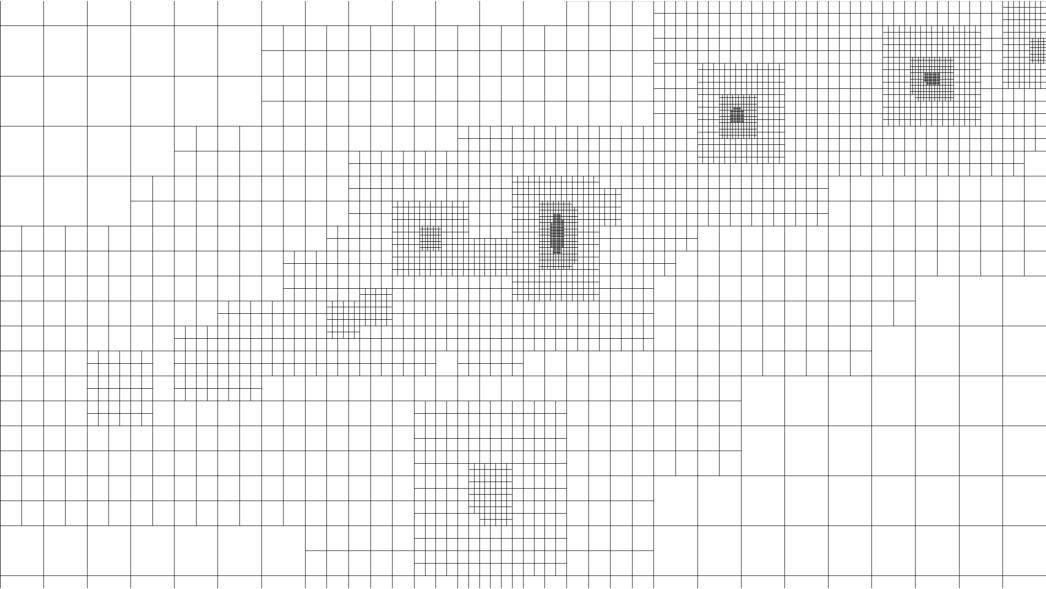
\includegraphics[width=.95\linewidth]{img/02/AMR.pdf} 
        \caption{Exemple de grille AMR. 
        La  résolution de la grille est augmentée dans les régions d'intérets.
}
 		\label{fig:AMR}
\end{figure}


\subsubsection{Octree}

Il existe deux grand groupe de maille adaptative.
Le premier groupe utilise des grilles fixes imbriquées %TODO ref

Le second est le groupe qu'utilise EMMA : fully threated tree description \citep{khokhlov_fully_1998-1}.
La base de cette représentation est de considérer que chaque cellule est associée a une grille 2x2x2 que l'on nommera un OCT (cf:\ref{lst:oct}), car décomposé en 8 sous parties qui sont elles même des cellules (cf:\ref{lst:cell}).
Et récursivement, chacune de ses sous parties peut a leurs tour être divisé ou non.
il en résultera un arbre nommé Octree.

\begin{figure}[bth]
        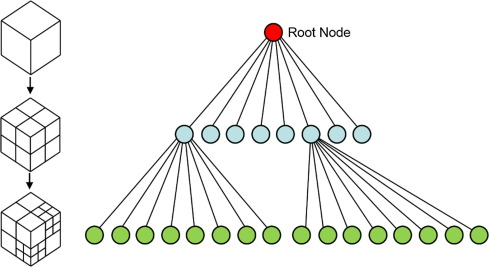
\includegraphics[width=.95\linewidth]{img/02/octree.jpg} 
        \caption{Représentation d'une grille AMR a gauche, et de son octree associé a droite. 
        Image extraite de \cite{SU201659}
}
 		\label{fig:octree}
\end{figure}

\subsubsection{Liste chainée}

Comme la grille est amenées a évoluer, il n'y a plus une position unique en mémoire associé à une position dans l'espace.
La grille est composée de cellules ordonnées sous forme de liste chainées.
Pour créer un lien entre elle, il est nécessaire de stocker l'information de voisinage.
Pour localiser un oct dans l'espace, on a besoin de stocker 2*D pointeurs vers les cellules voisine.
Un oct est également composé de d'un tableau de huit pointeurs vers ses huit cellules filles,  ainsi que d'un pointeur vers sa cellule mère.
On associera ensuite au cellules la partie physique (densité, pression, température, etc...).
Ainsi chaque cellule peut, sous certaine condition, etre subdivisée en un OCT pour augmenter la résolution localement.


On associera également les octs entre eux a l'aide d'une liste chainée. 
Il est nécessaire d'ajouter deux pointeurs a l'objet OCT : un vers l'oct précédent en mémoire et un vers l'oct suivant.

\begin{lstlisting}[float=bth,language=C,frame=tb,caption={les structures cellule de EMMA},label=lst:cell]
struct CELL{
  int id;            // permet de determiner la position de la cellule dans l'oct
  struct OCT *parent // l'oct pere de la cellule
  struct OCT *child; // si child est different de NULL alors la cellule est raffinee et child point vers l'oct enfant
  struct PHYSIC *data; // pointeur vers la partie physique
};
\end{lstlisting}

\begin{lstlisting}[float=bth,language=C,frame=tb,caption={les structures OCT  de EMMA},label=lst:oct]
struct OCT{
  struct CELL cell[8]; // les 8 cellules de l'oct
  struct CELL *nei[6]; // pointeurs sur les cellule voisines
  struct CELL *parent; // cellule mere
  struct OCT *next;    // oct suivant dans la liste chainee
  struct OCT *prev;    // oct precedent dans la liste chainee
  int level;           // niveau de l'oct
};
\end{lstlisting}


Terminologie:
On parlera de :

RACINE pour l'OCT de niveau 0. Il n'a pas de cellule mère et représente l'ensemble de l'espace de la grille.
La génération de conditions périodique (généralement utilisées en cosmologies) se fait de manière naturelle en faisant pointer tout les voisins de l'OCT racine vers lui même.


FEUILLE pour les cellules qui ne sont pas raffinées. 



\subsubsection{Gestion du raffinement}
\label{sec:raffinement}
%différentes condition de raffinement.\\
%sur la matière noire\\
%semi Lagrangienne\\
%sur le gradient d'ionization\\
%sur le gradient de densité (shock)\\

Il est possible de définir arbitrairement une condition de raffinement en fonction de la physique que l'on cherche a étudier.
Par exemple, dans des tests unitaires de type sphère de Stömgren ou explosion de Sedov, on marquera les cellules qui sont soumises a un gradient d'ionisation ou de densité supérieur a un certain seuil.
%TODO ajouter les ref des sections pour sedov et stromgren
Dans le cas de simulations cosmologique, on utilisera généralement une condition dite semi-Lagrangienne.
C'est a dire qu'une cellule sera marquée comme "a raffinée" si la masse de matière noire (ou de gaz) qu'elle contient est supérieur a huit fois la masse de matière noire (ou de gaz) moyenne d'une cellule de ce niveau.



En pratique, le raffinement se fera en trois temps:

\begin{itemize}
\item Dans un premier temps le code va passer en revue toutes les cellules d'un niveau, et les marquer comme "a raffiner" si une première condition physique est respectée.

\item Une fois tout le niveau passé en revue, le code va ensuite faire une série de $N_{buffer}$ passages sur tout le niveau en marquant à chaque fois les cellules voisine des cellules précédemment marquées.
Cette série de passage a pour but d’élargir la zone de raffinement et ainsi permettre une transition douce entre les niveaux.
Cette zone de $N_{buffer}$ cellules autour des zones soumises à la condition physique de raffinement sera appelée le "buffer de raffinement".

\item Une fois les cellules respectant ces deux conditions marquées, le raffinement est effectué.
\end{itemize}

En pratique le raffinement d'une cellule se fera en lui associant un OCT.
*child pointera alors vers le dernier OCT libre de la liste chaînée.

%le deraffinement
On remarquera que la condition de raffinement ne prends pas en compte le fait qu'une cellule soit déjà raffinée ou non.
Si une cellule est raffinée, mais qu'elle n'est pas marquée comme "a raffinée" elle sera donc dé-raffinée.

\subsubsection{Opérateurs de changement de grilles} \label{Opérateurs de changement de grilles}

Les opérations de raffinement/dé-raffinement font intervenir des opérateurs de changement de grille.
Le changement de résolution peut avoir lieu dans les deux sens :

\begin{itemize}
\item La \emph{restriction} consiste à dégrader la grille en résolution. La restriction la plus directe consiste à moyenner les cellules à dégrader. Par exemple, sur une grille à deux dimensions, pour diviser la résolution par deux, quatre cellules de la grille de départ devront être moyennées pour obtenir une nouvelle cellule de la grille à base résolution.

\item La \emph{prolongation} consiste à augmenter la résolution d'une grille, la prolongation la plus directe consiste à injecter les valeurs de l'ancienne grille dans un certain nombre de cellules de la nouvelle grille. (fig \ref{Opérateurs de changement de grille})
\end{itemize}

\begin{figure}[htbp]
\begin{center}
\subfloat[Restriction]{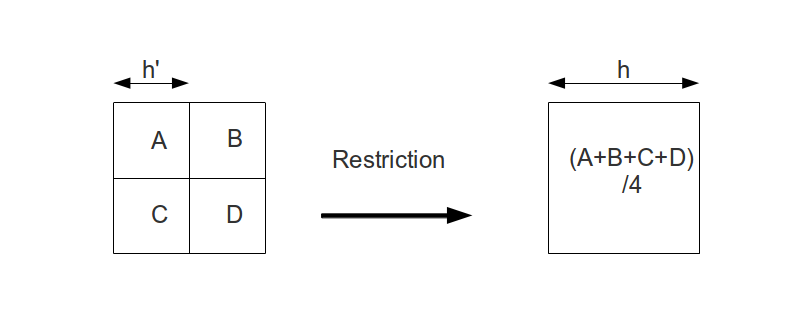
\includegraphics[width=.45\linewidth]{img/02/Restriction.png}}
\subfloat[Prolongation]{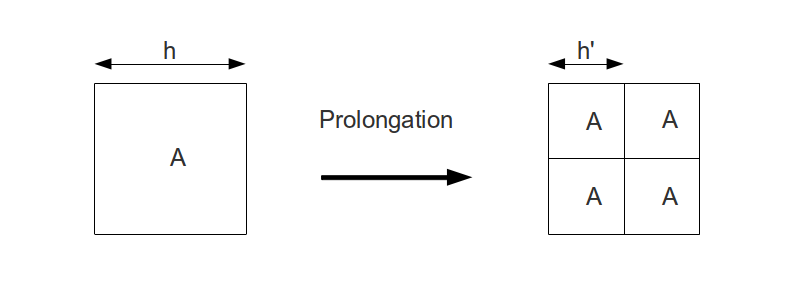
\includegraphics[width=.45\linewidth]{img/02/Prolongation.png}}\\
\subfloat[Niveau L  ]{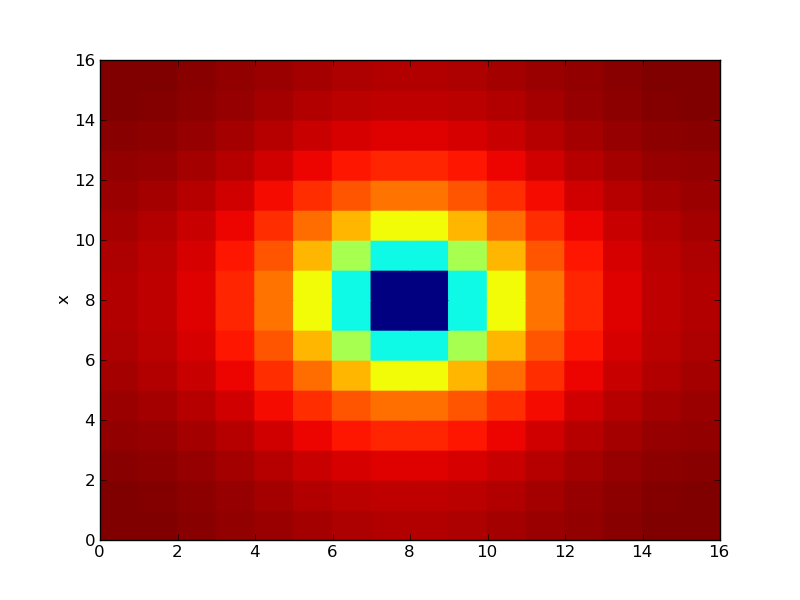
\includegraphics[width=.45\linewidth]{img/02/0090.png} \label{Opérateurs de changement de grille d}}
\subfloat[Niveau L+1]{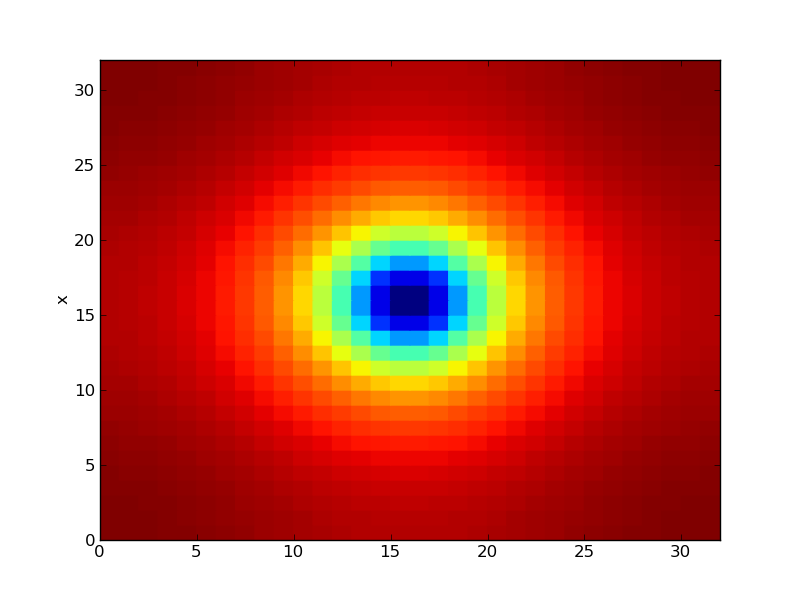
\includegraphics[width=.45\linewidth]{img/02/0088.png} \label{Opérateurs de changement de grille c}}
\caption{Opérateurs de changement de grille. 
Ils permettent de changer la résolution de la grille. Un exemple de restriction consiste à moyenner une valeur de plusieurs cellules, la prolongation associée consiste en une injection directe d'une valeur dans plusieurs cellules.}
\label{Opérateurs de changement de grille}
\end{center}
\end{figure}

La prolongation et la restriction sont des opérateurs aisément parallélisables. Chaque cellule (ou paquet de huit cellules) est indépendante des autres et il est possible de ne changer la résolution que d'une partie de la grille sans en affecter le reste.\\

Il existe principalement deux conditions sur les opérateurs de changement de grille. 
La première impose une certaine réciprocité entre eux, les opérateurs doivent être adjoints: il est nécessaire qu'après une prolongation, suivie d'une restriction la grille d'arrivée soit la même que la grille de départ. 
L'inverse n'est pas nécessairement vrai: après une restriction, de l'information est perdue et aucune prolongation ne pourra la recomposer.
La seconde condition concerne la precision des opérateurs, il est nécessaire que la somme des ordres des opérations soit supérieure à l'ordre de l'équation à résoudre. 
Ici, la restriction est d'ordre trois, la prolongation d'ordre un et le Laplacien d'ordre deux, cette condition est vérifiée.


\subsection{Recherche de voisin}
Nous verrons par la suite que l'état d'une cellule dépend des états des cellules qui l'entoure.
La recherche de voisins sera donc une étape importante dans la gestion de la grille.

La recherche de voisin se fera suivant ces étapes:

\begin{itemize}
\item en fonction de l'ID de la cellule, déterminer si la voisine est dans le même OCT parent.


\item
\begin{itemize}
\item Si c'est le cas, accéder a l'oct parent et a l'aide de l'indice du tableau de cellule, retrouver le voisin en question.
\item Si ce n'est pas le cas, accéder a la cellule mère de l'oct père et rechercher l'oct voisin
\end{itemize}

\end{itemize}


Nous avons vu dans la partie d'introduction a la physique de la reionisation que l'énergie noire représente la majore partie du contenu de l'univers.
Nous allons voir dans cette partie comme cette composante est simulée.

Bien que nous sachions absolument pas ce que peux être physiquement l'énergie noire, nous en observons les effets : l'Univers est en expansion accélérée.
Le solveur gérant l'énergie noire n'est pas a proprement parler un solveur numérique, mais plutôt d'un système d'unité. % servant a normaliser la physique.
Il consiste a normaliser les grandeurs par une variable fonction du facteur d'expansion.

% mais est la plus simple a simuler.
%Lien direct avec le facteur d'expansion (mettre ref section).

L'intégration de la cosmologie, régissant le lien en le temps et le facteur d'expansion sera réalisé une fois au moment de l'initialisation du code. %TODO ref
Il en résultera une table, conservée en mémoire pendant toute l'exécution.
Le facteur d'expansion sera alors interpoler dans cette table ne fonction de l'avancement de la simulation (cf partie calcul du pas de temps) %TODO ref

\subsection{Gestion de l'expansion}
Il existe deux possibilités pour modéliser l'expansion de l'univers a l'aide d'une grille.
La première consiste a considérer un élément de volume $dx$ de taille fixe, et au fur et a mesure que l'univers grandis, a y ajouter des éléments.
Le problème et que le coût numérique de la simulation croit, entre autre, avec le nombre d'éléments que l'on considère.
La seconde possibilité est de faire varier la taille des éléments de calcul avec le facteur d'expansion.
On appellera les longueurs ainsi exprimées des longueurs comobile.

\begin{equation}
r=a r'
\end{equation}

ou $r$ représente une longueur en unités physique et $r'$ en unités comobile.

Ainsi un cube de 10 Mpc physique de coté, pris aujourd'hui, aura une taille de 10 Mpc comobile (cMpc) aujourd'hui, mais aussi a redshift z=9 ou sa taille physique ne sera plus que de de 1Mpc physique.

De plus, il est généralement pratique de normaliser les grandeurs que l'on considère. 

\begin{equation}
r'=\tilde{r}r*
\end{equation}
ou $\tilde{r}$ est la longueur normalisée et $r*$ le facteur de normalisation.

La généralisation de ce principe a d'autre unités que la longueur est appeler système d'unités supercomobiles.
\citep{martel_convenient_1998}

\begin{table}[htbp]
\begin{center}
\begin{tabular}{r l} \hline 
Longueur: & $\tilde{r}=\frac{r}{ar_*}$ \\ \hline 
Densité de matière: & $\tilde{\rho}=\frac{\rho a^3}{\rho_*}$ \\ \hline 
Vitesse: & $ \tilde{v}=\frac{av}{v_*}$ \\ \hline 
Pas de temps: & $\tilde{dt}=\frac{dt}{a^2t_*}$\\ \hline 
Densité d’énergie potentielle: & $\tilde{\Phi}=\frac{a^2 \Phi}{\Phi_*}$\\ \hline 
Pression: & $\tilde{p}=\frac{a^5 p}{p_*}$\\ \hline 
Densité d’énergie cinétique: & $\tilde{\epsilon}=\frac{a^2 \epsilon}{\epsilon_*}$\\ \hline 
Densité D’éléments: & $\tilde{N}=a^3 N r_*^3$\\ \hline 
Flux: & $\tilde{F}=a^4 r_*^2 t_* F$\\ \hline 
\end{tabular} 
\end{center}
\caption{Passage du système d'unités physique vers le système d'unité supercomobile} 
\end{table}

\begin{table}[htbp]
\begin{center}
\begin{tabular}{r l} \hline 
Longueur  & $r_*=L$\\ \hline 
Densité & $\rho_* = \bar{\rho} = \frac{3H_0^2 \Omega_m}{8\pi G}$\\ \hline 
Temps & $t_* = \frac{2}{H_0 \sqrt{\Omega_m}}$\\ \hline 
Vitesse & $v_* = \frac{r_*}{t_*}$\\ \hline 
Potentiel & $\Phi_* = \frac{r_*^2}{t_*^2} = v_*^2$\\ \hline 
Pression & $p_* = \frac{\rho_* r_*^2}{t_*^2} = \rho_* v_*^2$\\ \hline 
Énergie & $\epsilon_* = \frac{p_*}{\rho_*} = v_*^2$\\ \hline 
\end{tabular} 
\end{center}

\caption{Facteurs de normalisation des différents grandeurs physique} 
\end{table}




\subsection{Gestion du pas de temps}


\begin{equation}
\frac{\delta a (\Delta t) } {a} < \epsilon
\end{equation}


\chapter{Les principaux solveurs physique}

Nous allons voir dans cette partie que plus une physique représente une part importante du contenu de l'Univers plus elle est simple et rapide a simuler.
Nous nous intéresserons a quatre solveurs distinct:
\begin{itemize}
\item d'énergie noire
\item de matière noire
\item du gaz
\item de la radiation
\end{itemize}
Et ce, dans un ordre décroissant d'importance, relativement a la quantité d'énergie totale.


%%%%%%%%%%%%%%%%%%%%%%%%%%%%%%%%%%%%%%%%%%%%%%%%%%%%%%%%%%%%%%%%%%%%%%%%%%%%%%%%%%%%%%%%%%%%%%%%%%%%%%%%%%%%%%%%%%%%%%%%%%%%%%%%%%%%%%%%%%%%%%%%



%%%%%%%%%%%%%%%%%%%%%%%%%%%%%%%%%%%%%%%%%%%%%%%%%%%%%%%%%%%%%%%%%%%%%%%%%%%%%%%%%%%%%%%%%%%%%%%%%%%%%%%%%%%%%%%%%%%%%%%%%%%%%%%%%%%%%%%%%%%%%%%%
\section{Matière noire}
\label{sec:solverDM}
La matière noire, dispose de propriétés de fluide non collisionelle, et se prête particulièrement bien a la représentation Lagrangienne, et donc a une simulation sous forme de particule.
Pour la simuler, on utilisera le principe des code Ncorp., c'est a dire qu'on utilisera un champs de particules massive interagissante par gravitation.
Ill existe différentes techniques pour suivre l'évolution d'un tel système.
Toutes sont basé sur le meme principe.
Les particules sont placée suivant une certaine condition initiale.
Et on cherche a connaitre la force gravitationnelle a laquelle chaque particule est soumise, dans le but de calculer son déplacement


\subsection{Génération des conditions initiales}

Nous avons vu %TODO ref
que le CMB nous donne de l'information sur l'état de la distribution de matière dans l'univers tres tot dans son histoire (il est possible de determiner le spectre de puissance des fluctuation de densité de l'univers primitif).
Le principe de la génération des condition iniales est d'utiliser ce spectre de puissance pour générer des surdensité repréentant statistiqument ces fluctuations.

Pour se faire on va générer une grille regulière sur laquelle on placera une particule au centre de chaque cellule.
Dans ce cas la densité est homogène.
On va alors perturber la position des particules de manière a respecter les fluctuations statistique observées dans le CMB.

Pour ce faire, il faut générer un bruit aléatoire Gaussien.
Tout les générateurs de condition initiales que j'ai pus rencontrer utilise une SEED aléatoire, dans le but de générer ce bruit aléatoire.
On convoluera ensuite ce bruit avec le spectre de puissance que l'on cherche a reproduire.

Et on appliquera les déplacement obtenus au particules.

Cette approximation n'est valable que dans le cas des petites perturbations, tant que l'on reste dans le régime linéaire.
Cette approximation du regime linéraire s'appelle l’approximation de Zeldovitch %TODO ref
\cite{2014MNRAS.439.3630W}


Plus l'on cherche a simuler des petites échelles, plus l'on sort vite du domaine de précision accéptable.
C'est pourquoi il est necessaire d'avoir recourt au simulations numériques.

Nous voyons ici que le spectre est limité des deux cotés.
D'un coté l'information des grandes échelles est tronquée par la taille de la boite considéré.
Il n'est pas possible d'avoir de l’information sur des longueurs d'onde du spectre plus grande que cette taille limite.
De l'autre coté, les petites échelles sont tronquées par la limite de résolution.
Le spectre est troqué au niveau de la longueur d'onde correspondant a la résolution de la grille.

Au passage cette perte d'information sur les hautes fréquences peux être problématique dans le cas ou la résolution est adaptative.
Dans le cas de l'AMR par exemple il peux paraître difficile d'autoriser un nombre élevé de niveau de raffinement puisque les niveaux nouvellement créer ne disposerons pas de l'information des conditions initiales.

En pratique j'ai principalement utilisé MUSIC et GRAPHIC %TODO ref.


%méthode
%gaussian random noise
%théorie des perturbation linéaire
%lien avec le spectre de puissance
%MUSIC et GRAPHIC
%limite la résolution min et max (min en masse et max en espace)


%une simulation est limité par sa taille et sa résolution -> ceci définit la plage d'échelle que l'on peut simuler
%
%principes de bases ennoncé dans Pen (1997) and Bertschinger (2001).
%
%    discrétisation de l'espace
%    placement des particules sur la grille
%    génération d'un bruit blanc
%    convolution avec un spectre de puissance connu (celui du CMB)

%
%\subsection{Théorie des perturbation linéaire}
%
%approximation de zeldovich
%perte de linéarité a un certain moment -> nécessité des simulation numériques





\subsection{Solveur de gravité}

A partir des condition initiales nouvellement générées, il faut ensuite suivre dynamiquement l'évolution des particules.

Je vais plus détailler le solveur de gravité que les autres puisque c'est celui sur lequel j'ai le plus travaillé.
%Le sloveur que je connais le mieux.
%Fluide non collisionnel -> particule\\

On cherche a obtenir la position des particules a chaque instant.
Pour cela, il nous faut leurs vitesses.
Pour cela, il nous faut leurs accélération.
Pour cela, il nous faut la force qui leur est appliquée.

Ce système d'équation est appelé le système d'équation de Vlasov-Poisson :

\begin{equation}
\begin{cases}

\frac{d{x}_p}{dt} = { v}_p, \\
\frac{d{ v}_p}{dt} = -\nabla \phi , \\
\Delta \phi= 4\pi G \rho.

\end{cases}
\label{eq:Ncorps}
\end{equation}

Il existe plusieurs méthodes pour résoudre ce système.
Historiquement la première méthode était le méthode :

\paragraph{Particule-Particule : } c'est le méthode la plus directe pour calculer l'évolution d'un fluide non collisionnel. 
Elle consiste, pour chaque particule, a sommer les contribution gravitationnelles de toutes les autres particules.
Ce type de code dispose d'une très bonne précision mais la quantité de calcule évolue en ordre $O(N^2)$, ce qui fait que ce type de code est très coûteux.

\begin{equation}
\vec{F}_i=-\sum_{j\neq i} G \frac{G m_i m_j(\vec{r}_i - \vec{r}_j) }{ |\vec{r}_i - \vec{r}_j |^3}
\end{equation}

Une évolution de cette méthode est la méthode :

\paragraph{Particule-tree : } elle  consiste a regrouper les particules loin de la particule courante en un amas aillant une interaction gravitationnelle commune
% (Barnes & Hut 1986) 
Cette approximation permet de limiter considérablement le nombre de calcul pour les interactions lointaine qui sont de toute façons faibles.


Une autre méthode, celle qui nous intéresse ici consiste a utiliser le potentiel:

%On peux obtenir cette force soit par calcul direct, soit par dérivation du potentiel.

\begin{equation}
\vec{F}=-\Delta \Phi
\end{equation}

Le potentielle sera calculé sur une grille, cette méthode sera nommée :
\paragraph{Particule-Mesh : } on projette les particules sur une grille
ENZO %code, Bryan & Norman 1998
RAMSES

La méthode de projection des particules sur la grille n'est pas unique.
On peut par exemple se contenter d'ajouter la masse de la particule dans la cellule a laquelle elle appartient.
Cela donne un résultat très bruité.
Une méthode d'ordre supérieure est appelé Cloud in cell (CIC)

\paragraph{Cloud in cell : } Le CIC consiste a considérer une étendue spatiale aux particules et a pondérée la masse appliqué au cellule par l'intersection de de son volume et de celui de la cellule.
Fig\,\ref{fig:CIC}.
On associe généralement une taille a la particule similaire a celle des cellule sur laquelle on la projette.
Dans le cas ou L’étendue de la particule intersecte des cellules de différents niveaux on lui associera la taille de la plus grande cellule dans le but de lisser la transition entre les niveaux.


\begin{figure}[bth]
		\centering
        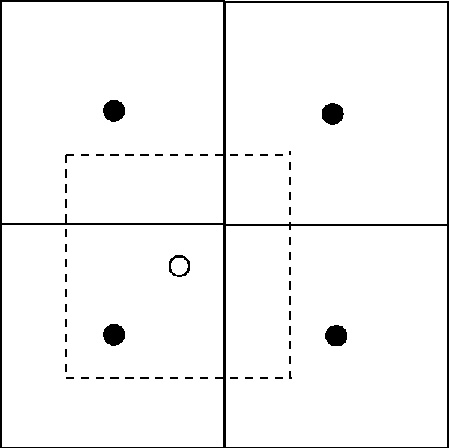
\includegraphics[width=.5\linewidth]{img/02/CIC.jpg} 
        \caption{Représentation en 2D du Cloud In Cell. 
        La masse d'une particule est répartie dans le cellules environnantes en lui associant une étendue spatiale.
        %http://homepage.univie.ac.at/franz.vesely/cp_tut/nol2h/new/c6sm_s4lr.html
}
 		\label{fig:CIC}
\end{figure}

Il existe des méthodes d'ordre supérieur avec des kernel plus complexe que le top-hat du CIC comme par exemple des kernel en triangle ou en gaussienne.
%http://techfinder.stanford.edu/technology_detail.php?ID=30866

Une fois la grille de densité générée nous pouvons calculer le potentiel.

\subsubsection{l'équation de Poisson}
\begin{equation}
\Delta \Phi = 4 \pi G \rho
\end{equation}

qui devient en système d'unité supercomobile:
\begin{equation}
\Delta \Phi = 6 a \delta
\end{equation}
avec le contraste de densité: 
\begin{equation}
\delta = \tilde{\rho} / < \tilde{\rho} > - 1 
\end{equation}

integration de l'equation de Poisson pour obtenir le potentiel
\begin{equation}
\Delta \phi = 4\pi G \rho \longrightarrow \phi = \iint \Delta \phi = \iint 4\pi G \rho
\end{equation}

Pour cela, il existe principalement deux types de méthodes. La première est basée sur les Transformées de Fourier. Cette méthode, très rapide, utilise le fait que dans l'espace de Fourier, une intégrale se résume à une division par un nombre d'onde. Déterminer le champ de potentiel revient à : 
\begin{itemize}
\item Effectuer la transformée de Fourier de la densité
\item Diviser par $k^2$
\item Effectuer la transformée de Fourier inverse
\end{itemize}

\begin{equation}
\rho_{(\vec{x})} \overset{FFT}{\longrightarrow}  \rho_{(\vec{k})} \times \frac{1}{k^2}  \overset{RFFT}{\longrightarrow}  \phi_{(\vec{x})}
\end{equation}

De par la nature des transformées de Fourier, le champ de densité doit être périodique pour que l'implémentation de cette technique ne se révèle pas trop complexe. Ce qui n'est pas un problème en simulation cosmologique, où les conditions de bords sont toujours périodiques mais est plus problématique lors de la simulation de structures isolées, telles les galaxies ou les amas de galaxies. Ensuite, les FFT nécessitent un échantillonnage régulier ce qui implique que cette méthode est incompatible avec les grilles adaptatives. Et dernièrement, le passage dans l'espace des fréquences nécessite des conditions de types plans parallèles lors parallélisation, conditions incompatible avec la gestion de grille utilisé par les code AMR dont \emph{Quartz} fait partie. \\

Un autre type de méthode de résolution possible est une méthode itérative. Elle consiste à faire converger le potentiel à partir d'une condition initiale arbitraire. Ce type de méthode est plus lente que la méthode par FFT mais  permet d'utiliser tout type de conditions de bords, d'être facilement parallélisable et surtout est compatible avec les méthodes basées sur des grilles adaptatives. PAr la suite, c'est donc une méthode itérative et plus précisément une méthode \emph{Multigrille} qui à été développée.\\

Le potentiel est alors dérivé pour obtenir la force ressentie dans chaque cellule. Il est ensuite aisé de calculer l'accélération subie par les particules de chaque cellule, et par intégration temporelle, leurs nouvelles positions et vitesses.

Par analogie à l'équation de la chaleur par exemple, la densité correspond aux sources chaudes et le potentiel à la température, à $t=0$ les sources chaudes sont allumées et la chaleur se propage jusqu'a ce que le milieu ait atteint sa température d'équilibre. Ici, c'est donc la gravité qui se diffuse dans le milieu. \\


\begin{equation}
\dfrac{\partial \phi}{\partial t} = \Delta \Phi -S 
\end{equation}


\subsubsection{Méthode jacobi}


La méthode de Jacobi est la façon la plus simple de relaxer ce type d'équation, elle consiste à utiliser directement la forme discrète de l'équation de Poisson modifiée. L'équation à intégrer est:

\[ \dfrac{\phi^{t+1}_i - \phi^{t}_i}{\Delta t}  =  \Delta \phi_i^t - 4 \pi G \rho^t_i \]

où, à 3 dimensions, le Laplacien s'exprime :

\[ \Delta \phi_i^t = \dfrac{\phi_{x+1,y,z}^t  + \phi_{x-1,y,z}^t + \phi_{x,y+1,z}^t  + \phi_{x,y-1,z}^t + \phi_{x,y,z+1}^t + \phi_{x,y,z-1}^t	- 6\phi_{x,y,z}^t}{\Delta x ^2} \]
		
Le principal avantage de cette méthode est sa parallélisation triviale. 
Elle ne nécessite de connaître l'état du système qu'au temps $t$. 
Ansi, chaque fils d'exécution parallèle (thread) est indépendant et n'a pas d'information à communiquer aux autres .



\subsubsection{Gauss Seidel}
Gauss-Seidel est une amélioration de Jacobi. Au lieu d'utiliser, à chaque pas de temps, les valeurs de la grille au niveau précédent, cette méthode consiste à toujours utiliser la valeur la plus à jour disponible. Une fois $\phi^{t+1}_0$ calculé à l'aide de $\phi^{t}_i$, la valeur de $\phi^{t+1}_1$ n'est pas calculée à l'aide de $\phi^{t}_0$ mais avec $\phi^{t+1}_0$. En utilisant toujours la valeur la mieux estimée, cette méthode accélère la convergence. L'intégration temporelle ne change pas, mais l'intégration spatiale devient: 

\[ \Delta \phi_i^t = \dfrac{\phi_{x+1,y,z}^t  + \phi_{x-1,y,z}^\mathbf{t+1} + \phi_{x,y+1,z}^t  + \phi_{x,y-1,z}^\mathbf{t+1} + \phi_{x,y,z+1}^t + \phi_{x,y,z-1}^\mathbf{t+1}	- 6\phi_{x,y,z}^t}{\Delta x ^2} \]

La parallélisation de cette méthode est plus compliquée que dans le cas de Jacobi. La détermination de la valeur de chaque cellule nécessite de connaître l'état le plus à jour de ses voisins et donc de faire passer de l'information entre les threads.
 Cependant, une méthode nommée Gauss-Seidel Rouge-Noir permet une parallélisation sur multiprocesseurs en séparant l'espace en un damier de couleurs. Chaque processeur ne calcule alors qu'une seule couleur. Le premier processeur calcul par exemple les cases blanches de l'échiquier à partir de $\phi_i^t$, puis le second calcul le cases noires à partir des cases blanches déterminé par le premier.


\subsubsection{Sur-relaxation successive (SOR)}
La méthode de sur-relaxation successive consiste à appliquer un coefficient à la méthode de Gauss-Seidel (ou de Jacobi, en fonction de la méthode de dérivation spatiale) pour sur-estimer l'évolution de la convergence et ainsi l'accélérer. l'équation à intégrer devient:
\[ \phi^{t+1}_i = \phi^{t}_i + \omega  \Delta t \left (\Delta \phi_i^t - 4 \pi G \rho^t_i \right )  \]
où $\omega \in \left] 0,2 \right [$ est le paramètre de sur-relaxation.
\begin{itemize}
\item lorsque $\omega <1$ La méthode est dite de sous relaxation.
\item lorsque $\omega =1$ La méthode devient celle de Gauss-Seidel.
\item lorsque $\omega >1$ La méthode est dite de sur relaxation.
\end{itemize}
Il existe des moyens analytiques pour déterminer la valeur optimale de $\omega$ mais très souvent cette valeur est déterminée empiriquement à partir d'une série de tests. $\omega = 1,2$ est très souvent utilisé.
%L'expression de cette méthode apparait généralement dans la litterature sous la forme:


\subsubsection{Condition d'arrêt}
Ces méthodes sont itérées jusqu’à ce qu'un certain critère convergence soit respecté. Le critère le plus couramment utilisé consiste à mesurer l'évolution de la convergence en comparant sa valeur au temps $t$ à celle au temps $t+1$.
\[ \phi^{t+1}_i - \phi^{t}_i < \epsilon \]
ou, de manière équivalente:
\[ \Delta \phi_i^t - 4 \pi G \rho^t_i< \epsilon \]

Pour prendre en compte la possibilité que le potentiel ait convergé sur une partie du domaine seulement, et pour ne pas stopper le processus trop tôt, c'est le module de cette expression qui est considéré. De plus il est d'usage de normaliser ce module par la source que l'on considère.

\[\dfrac{ \sqrt{  \sum_i \left (  \Delta \phi_i^t \right )^2 - \left (4 \pi G \rho^t_i  \right )^2 } }{\sqrt{  \sum_i  \left (4 \pi G \rho^t_i  \right )^2 } } < \epsilon \]

A cette condition est ajouté un nombre d'itérations maximum fixe pour éviter les problèmes de boucles infinies lorsque le potentiel n'arrive pas à converger (oscillation autour d'une valeur d'équilibre par exemple).

\subsubsection{Multigrille}
Cette seconde technique, plus efficace encore, consiste à travailler non pas sur la grandeur elle même, mais sur l'erreur effectuée dans l'estimation de cette grandeur.

Elle utilise la linéarité de l'opérateur Laplacien: 
 
Si l'équation à résoudre est de la forme : 
\[ \mathcal{L} u = f \]
Sa forme discrète est :
\[ \mathcal{L}_h u_h = f_h \]
si $\tilde{u_h}$ correspond à une estimation de la solution et $u_h$ à la solution exacte, l'erreur est alors la différence entre les deux : 
\[ v_h = u_h - \tilde{u_h} \]
le résidu est défini comme:
\[ d_h = \mathcal{L}_h \tilde{u_h} - f_h \]
comme $\mathcal{L}_h$ est linéaire:
\[ \mathcal{L}_h u_h = \mathcal{L}_h (v_h + \tilde{u_h} ) = \mathcal{L}_h v_h +\mathcal{L}_h \tilde{u_h} \]
\[ f_h   = \mathcal{L}_h \tilde{u_h} - d_h\]
et finalement :
\[ \mathcal{L}_h v_h = -d_h \]

L'équation à résoudre est alors modifiée en considérant que l'inconnue n'est plus le potentiel mais l'erreur commise sur son estimation. Le terme source n'est plus la densité mais la densité moins son estimation grossière.\\


Le cycle consiste à lisser (relaxer quelques fois) le potentiel à pleine résolution, les petites échelles vont alors rapidement converger, à calculer ensuite l'erreur commise à ce stade. L'erreur est dégradée à plus basse résolution, elle ne contient alors que de l'information sur les basses fréquences de la grille de départ, les hautes fréquences de la grille à pleine résolution ont été supprimées par la dégradation. Cette perte d'information sur les hautes fréquences n'est pas problématique car les hautes fréquences ont déjà convergé l'erreur est donc petite (voir nulle) aux hautes fréquence et est maximale aux basses. Les hautes fréquences de cette nouvelle grille correspondent alors à des fréquences plus basses et donc plus difficiles à faire converger sur le grille globale. La solution exacte de l'équation de l'erreur est calculée par itération (relaxée jusqu'a convergence) à partir des résidus sur cette petite grille. Le potentiel précédemment estimé est alors corrigé de l'erreur exacte interpolée à pleine résolution en utilisant:
\[ \tilde{u}_h^{new} = \tilde{u_h} + v_h \]
Le potentiel corrigé est alors lissé par quelques dernières itérations.\\

Ce cycle peut être résumé ainsi:


\begin{tabular}{ll}
Lisser 		& 	$ \mathcal{L} u_h = f_h $\\
Calculer	&	$ d_h = \mathcal{L}_h \tilde{u_h} - f_h $\\
Restreindre	&	$ d_H = Rd_h$\\
Résoudre	&	$ \mathcal{L} v_H = -d_H $\\
Interpoler	&	$ v_h = Pv_H$\\
Corriger	&	$ \tilde{u}_h^{new} = \tilde{u_h} + v_h$\\
Lisser		&	$ \mathcal{L} u_h = f_h $
\end{tabular} 



A partir de la méthode deux grilles, rien n'empêche d'estimer l'erreur sur l'erreur par la même méthode, ce processus peut être utilisé récursivement pour générer tout un ensemble de sous grilles et ainsi accélérer encore la convergence.\\

L'algorithme devient alors:\\

MG(level, $u_h$, $f_h$)
\begin{itemize}	
\item 	si level = level min:
\item[]	\begin{tabular}{ll}
		Résoudre & $\mathcal{L} u_h = f_h $
		\end{tabular}
\item 	sinon:
\item[]	\begin{tabular}{ll}
		Lisser 		& 	$ \mathcal{L} u_h = f_h $\\
		Calculer	&	$ d_h = \mathcal{L}_h \tilde{u_h} - f_h $\\
		Restreindre	&	$ d_H = Rd_h$\\
		Appeler 	&	MG(level-1, $v_H$, $-d_H$) \\
		Interpoler	&	$ v_h = Pv_H$\\
		Corriger	&	$ \tilde{u}_h^{new} = \tilde{u_h} + v_h$\\
		Lisser		&	$ \mathcal{L} u_h = f_h $
		\end{tabular} 
\end{itemize}

Où la taille de la grille au niveau "level" est de $2^{3level}$ ( si level = 9, la taille de la grille est de $512^3$ ). $h$ est le pas de la grille au niveau "level" et $H = 2h$. Les opérateurs $P$ et $R$ sont les opérateurs de prolongation et de restriction explicité section \ref{Opérateurs de changement de grilles}
Cet algorithme est représenté graphiquement sur la figure \ref{Description du V-cycle}.


\begin{figure}[htbp]
\begin{center}
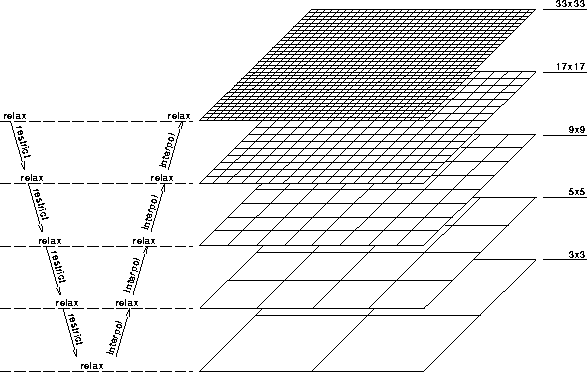
\includegraphics[scale=0.35]{img/02/multigrid.png}
\caption{\textbf{Vue des différents niveaux de grilles.} Image extraite de \href{http://MGNet.org}{MGNet.org} }
\label{Vue des différents niveaux de grilles}
\end{center}
\end{figure}	

\begin{figure}[htbp]
\begin{center}
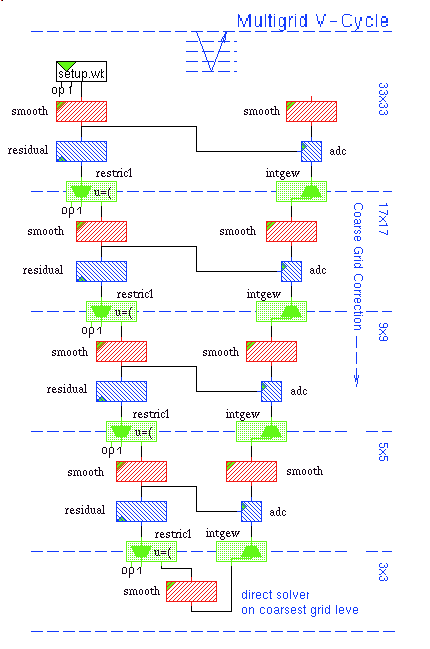
\includegraphics[scale=0.35]{img/02/Vcycle.png}
\caption{\textbf{Description du V-cycle.} Image extraite de \href{http://MGNet.org}{MGNet.org}}
\label{Description du V-cycle}
\end{center}
\end{figure}		

En jouant sur le nombre d'appels récursifs de la fonction, il est possible de créer différentes géométries de cycles. 
Un seul appel génère un cycle nommé cycle en V (fig. \ref{Description du V-cycle}), deux un cycle en W, etc... 

\subsection{Implémentation dans EMMA}
Dans EMMA, la potentiel est calculé par multigrille sur la grille coarse, et par Jacobi sur les niveaux raffinés.
La solution de la grille coarse étant injectée sur les niveau suivant, la solution est deja anticipée. 
Il en résulte une convergence rapide.

On prendra garde, lors de calcul en parallèle, a utiliser un niveau minimum de telle sorte que chaque processeurs dispose au minimum d'un oct.
Dans le cas contraire, le calcul ne donnera pas le bon résultat.

\subsection{Liste chaînée de particule}
La gestion des particules dans EMMA utilise le principe de la liste chaînée déjà abordée pour les OCT. %TODO ref
A chaque cellule est associée  un pointeur vers une particule de tète.
Si ce pointeur est NULL, la cellule ne contient pas de particule.
Les particules entrant dans cette cellule seront ajoutées a la liste chaînée.
On prendra garde a gérer cette liste au moment du raffinement et du déraffinement des cellules.



\subsection{Le pas de temps}

Le pas de temps sera calculer de telle sorte a respecter la condition de Courant.
Une particule ne doit pas se déplacer de plus d'une fraction de case a chaque pas de temps.


%	    dtloc=0.1*SQRT(2.*M_PI/(3.*(curoct->cell[icell].gdata.d+1.)*aexp));
%\begin{equation}
%
%\end{equation}



%%%%%%%%%%%%%%%%%%%%%%%%%%%%%%%%%%%%%%%%%%%%%%%%%%%%%%%%%%%%%%%%%%%%%%%%%%%%%%%%%%%%%%%%%%%%%%%%%%%%%%%%%%%%%%%%%%%%%%%%%%%%%%%%%%%%%%%%%%%%%%%%

\clearpage
\section{Le solveur hydrodynamique et la physique baryonique}

%solveur hydro
%partie la plus intensive en calcul


En cosmologie, le gaz est principalement soumis a deux forces : la pression et la gravité.
Comme nous l'avons vu plus tot, L'Univers est consitué d'une grande quantité d'Hydrogene et d'Helium sous forme gaseuse.
La physique du gaz est régie par les equations d'Euler auto-gravitantes :

\begin{equation}
\begin{cases}

{ \frac{ \partial \rho }{ \partial t } + \nabla \cdot (\rho v) = 0}, \\
\\
{ \frac{ \partial }{ \partial t } (\rho v) + \nabla \cdot (\rho v \otimes v ) \nabla p = -\rho\nabla \phi }, \\
\\
{ \frac{ \partial e }{ \partial t } + \nabla \cdot [ \rho v (e+p/\rho) ] = -\rho v \cdot \nabla \phi },

\end{cases}
\end{equation}
\label{eq:hydro}

Ce set d'équation peut être réécris sous la forme:

\begin{equation}
U+F(U) = 0,
\end{equation}

avec:
\begin{equation}
U=
\begin{cases}
{ \rho}\\
{ u}\\
{ v}\\
{ w}\\
{ E}
\end{cases}
,
F(U)=
\begin{cases}
{ \rho u}\\
{ \rho u^2+p}\\
{ \rho uv}\\
{ \rho uw}\\
{ u(E+p)}
\end{cases}
\end{equation}

Pour suivre l'évolution de ce gas nous allons le considérer comme parfait et monoatomique.

L’équation d'état du gaz sera donc:
\begin{equation}
p=\rho k T, 
\end{equation}
avec $k=1.38064852 \cdot 10^{-23} \left[ \mathrm{m^2 \cdot kg \cdot s^{-2} \cdot K^{-1}} \right] $ la constante de Boltzmann.


\subsection{Le probleme de Riemann}
L'idée est de décomposer le domaine en cellules dans lesquelles les grandeurs seront localement constantes. (Piecewise constant approximation)
On utilisera ensuite les equations d'Euler pour résoudre localement le problème de Riemann a chaque interfaces de cellule.
Nous aurons donc accès aux flux de matière et d'énergie entre les cellules pour pouvoir calculer l'état suivant  


Le problème de Riemann consiste a considérer l’évolution d'un system d’équation différentielles a partir d'une condition initiale.
En aillant l’état d'un système régis par des equations différentielles un instant donné, qu'elle sera sont évolution?

\begin{itemize}
\item PDE
\item IC
\item BC
\end{itemize}

\subsection{La discretisation du probleme.}


Contrairement a la résolution de l’équation de Poisson, il n'est plus possible d'utiliser une discrétisation des dérivées a l'aide d'un différence finie centrée.
Nous allons rapidement voir pourquoi dans cette section.


Une différence finie centrée peut être décomposée en deux différence finies : 
\begin{equation}
\frac{d u}{dx} \approx \frac{u_{i+1}  + u_i}{\Delta x} 
\end{equation}

\begin{equation}
\frac{d u}{dx} \approx \frac{u_i  + u_{i+1}}{\Delta x} 
\end{equation}



Considérons que nous voulons résoudre l'équation :
\begin{equation}
\frac{du}{dt} + a\frac{du}{dx} = 0
\end{equation}

Dans le premier cas, la discrétisation pourra s'écrire : 
%la propagation d'une onde a la vitesse $a$ pourra être discrétisée en utilisant.


\begin{equation}
\frac{u_i^{t+1} + u_i^t }{\Delta t}   +a \frac{u_{i+1}^t  + u_i^t}{\Delta x} = 0
\end{equation}


\begin{equation}
u_i^{t+1}  = u_i^t +  c \left( u_{i+1}^t  + u_i^t \right) 
\end{equation}

ou : 

\begin{equation}
c= \frac{a \Delta t}{\Delta x},
\end{equation}
est le nombre de Courant


A l'aide d'une analyse de von-Neumann (cf \cite{toro1999riemann}), on montre que la stabilité de ce schéma dépend du signe de a, la vitesse de propagation de l'onde.

\begin{itemize}
\item si a est positif, ce schéma est conditionnellement stable (la condition étant que la condition de Courant soient respectée : $0<c<1$) .
Ce schema est appélé méthode UPWIND.

\item A l'inverse on montre que que dans le cas de la seconde différence finie, le schéma est inconditionnellement instable. 
Ce shema est appelée méthode DOWNWIND.
\end{itemize}

Seule la méthode upwind permet de suivre correctement la propagation d'onde.
Le problème est qu'a trois dimension, il est impossible de respecter cette condition pour un système quelconque.
% déterminer dans quelle direction se propage une onde quelconques.


De plus il a été montré que cette méthode n'est pas conservative, et qu'elle était incapable de suivre les chocs (fortes discontinuités)

\subsection{Méthode de Godunov}


Godunov  \cite{MR0119433} a répondu a ce problème.

methodes conservative

introduction aux volumes finis
consiste a estimer le flux aux interfaces des cellules.


%\subsection{discretisation}
\begin{equation}
 \frac{\partial U}{\partial t} + \nabla \cdot (F(U)) = S(U), 
\label{eq:rad_generale}
\end{equation}

avec $U$ le vecteur des quantité conservées, $F$ la fonction de flux, et $S$ le terme source. Pour la résolution du transport des photons (sans terme source), on retrouve :

\begin{equation}
\frac{ u^{t+1}_i - u^t_i }{\Delta t} + \frac{ F^t_{i+1/2} - F^t_{i-1/2} }{\Delta x} =0,
\label{eq:rad_solver}
\end{equation}

ou $F^t_{i+1/2}$ et $F^t_{i-1/2}$ sont les flux numérique intercellules, une estimations des flux physique.

$F^t_{i+1/2}$

\subsection{Méhtode HLL et HLLC }
La méthode de HLL Harten, Lax et van Leer 
recalculation des flux entre les cellules

\subsection{MUSCL}
Monotonic Upstream-Centered Scheme for Conservation Laws (van Leer, 1979)
Consiste a considerer une valeur dans la cellule, non plus constante mais variable.
Cette variation est interpolée linéairement
%En utilisant la méthode de pente.

\subsection{Minmod}



\subsection{Le pas de temps}

Le pas de temps respecte encore une fois la condition de courant.

\begin{equation}
\frac{dx * CFL }{3*(max(v) + c_s)}
\end{equation}

avec $cs = \gamma P/\rho$

%%%%%%%%%%%%%%%%%%%%%%%%%%%%%%%%%%%%%%%%%%%%%%%%%%%%%%%%%%%%%%%%%%%%%%%%%%%%%%%%%%%%%%%%%%%%%%%%%%%%%%%%%%%%%%%%%%%%%%%%%%%%%%%%%%%%%%%%%%%%%%%%
\section{Le solveur radiatif}
\label{sec:rad_solver}

Il existe deux grandes famille de code de transfert de rayonnement.
\begin{itemize}
\item La première famille utilise une représentation très physique de la lumière, et simule la radiation a l'aide de rayons se propageant dans l'espace.
CRASH \citep{2003MNRAS.345..379M}, C$^2$RAY\citep{2006NewA...11..374M}.
Ce type de code utilise une principe qui se rapproche physiquement de la vraie nature de la lumière.
Chaque source lance un certain nombre de groupe de photon, qui vont se propager et interagir avec le milieu.
Plus les sources sont nombreuses, plus le nombre de groupe de photons a suivre devient important, et plus le cout numérique l'est également.

\item La seconde, celle utilisée dans EMMA, repose sur le principe de considérer la lumière comme un fluide. \citep{gnedin_multi-dimensional_2001, aubert_radiative_2008}.
Ces méthodes dites méthodes aux moments utiliseront donc les même concepts que le solveur hydrodynamique, mais avec un système initial d'équations différentes. 
EMMA utilise une approximation du moment au premier ordre, son solveur repose sur l'\textit{approximation M1} \citep{levermore_relating_1984}.
Son principal avantage est que le coût numérique est indépendant du nombre de sources.
\end{itemize}

Ce solveur se déroule en deux temps.
Premièrement, il faut calculer la propagation du rayonnement, on appelles cette étape \textit{le transport} des photons.
Deuxièmement, il faut le couplage entre le rayonnement et le gaz, c'est a dire calculer l'impact \textit{chimie} du gaz.


\subsection{Les équations du transfert du rayonnement}
\begin{equation}
\frac{1}{c} \frac{\partial I_\nu}{\partial t} + \vec{n}\cdot \vec{\nabla} I_\nu = \eta_\nu - \kappa_\nu I_\nu 
\end{equation}
Avec: $I_\nu(\vec{x},\vec{n},t)$ l'intensité spécifique,
$\eta_\nu(\vec{x},\vec{n},t)$ la source de rayonnement,
le coefficient d'absorption $\kappa_\nu(\vec{x},\vec{n},t) = \sigma_\nu n_H$, 
$\sigma_\nu$ la section efficace de photo-ionisation de l'hydrogène neutre et $n_H$ la densité d'hydrogène neutre


\begin{equation}
\begin{cases}

\frac{ \partial N_\nu }{ \partial t } + \vec{\nabla} \cdot \vec{F}_\nu = -\kappa_\nu c  N_\nu + S_\nu,\\

\frac{ \partial \vec{F} }{ \partial t } + c^2 \vec{\nabla} P_\nu = -\kappa_\nu c \vec{F}_\nu ,

\end{cases}
\label{eq:densite_energie}
\end{equation}
Représentant respectivement les moments d'ordre 0 et 1 de $I_\nu$ avec:
$\vec{F}_\nu$ le flux radiatif, 
$P_\nu $ la pression radiative
et $S_\nu = \dot{N}_\nu^* + \dot{N}_\nu^{rec}$ le taux d’émission de photon due aux sources $\dot{N}_\nu^*$ et a la recombinaison $ \dot{N}_\nu^{rec}$


\subsection{Relation de fermeture et approximation M1}
La fermeture du système se fait par l’intermédiaire de l’équation d’état, avec $D$ le tenseur d’Eddington :

\begin{equation}
 P_\nu = D N\nu ,
\label{eq:fermeture}
\end{equation}

où D est approximé par le modèle M1 \citep{levermore_relating_1984}%,gonzalez2005} :

\begin{equation}
\begin{cases}

D = \frac{ 3\chi -1 }{2} \mathbb{1} + \frac{ 1 - \chi }{2} \vec{n} \otimes \vec{n} , \\
\\
\chi(\vec{f}_\nu) = \frac{ 3+4 |\vec{f}_\nu|^2 }{5+2\sqrt{4-3|\vec{f}_\nu|^2}} , \\
\\
\vec{f}_\nu = \frac{ \vec{F}_\nu }{c N\nu }  ,

\end{cases}
\label{eq:tenseur}
\end{equation}


\subsection{Pas de temps et vitesse de la lumière réduite}

Condition de Courant radiative : $ c \leq \Delta x / \Delta t $.
Le pas de temps est donc plusieurs ordres de grandeur plus petit que celui de l'hydrodynamique.

%Pour compenser cette 

Les simulation cosmologique utilise l'approximation Newtonienne: les processus entrant en jeux on des vitesses très inférieurs a celle de la lumière.
L'idée est de diminuer la vitesse de la lumière dans le code tout en restant dans le domaine de l'approximation newtonienne.
Cette idée est développée en détails dans la section %TODO ref



\subsection{La chimie}

La chimie fait le lien entre le solveur radiatif et le solveur hydrodynamique.
C'est a ce moment qu'est appliquée l'énergie apportée par la radiation au gaz.
gestion du refroidissement/ de la température/ énergie interne
Contrairement au transport, la chimie est non conservative.

Densité de photons
\begin{equation}
\frac{dN}{dt} = S - c \sigma_N n_H N + \left( \alpha_A(T)  - \alpha_B(T) \right) x^2n_0^2
\end{equation}

Flux de photons
\begin{equation}
\frac{dF}{dt} = - c \sigma_N n_H F
\end{equation}

État d'ionisation
\begin{equation}
\frac{dn_H}{dt} =  \left( \alpha_A(T)x^2  - \alpha_B(T)x (1-x) \right) n_0^2 - c \sigma_N n_HN
\end{equation}


Énergie interne
\begin{equation}
\frac{de}{dt} = c n_H \Sigma_E N - \Lambda_{(n_0,x,T)}
\end{equation}


Les taux de réaction chimique $\alpha_A(T)$, $\alpha_B(T)$ et $\beta_(T)$ sont repris de tables de \cite{theuns_p^3m-sph_1998}.
Les sections efficace d'interactions viennent de \cite{hui_equation_1997}.

Les processus chimique agissant sur des échelles de temps courtes par rapport au transport des photons, le pas de temps sera plusieurs ordres de grandeurs plus faible.
En pratique, a chaque pas de temps radiatif, on effectuera un sous-cyclage sur le pas de temps chimique.
Après chaque pas de temps chimique, la variation d’énergie est calculée. 
Si celle ci est supérieure a 10\%, le pas de temps est divisée par 2 et l'étape courante est recalculée. (cf \cite{rosdahl_ramsesrt_2013}) 

Étant donné que le processus chimique sont uniquement local (ils ne dépendent pas de l'état des cellules voisines) et que la quantité de calcul est relativement importante, le portage du solveur chimique sur GPU est très intéressant du point de vue accélération.


\subsection{Groupes de photons}
\label{sec:groupedephotons}

Il n'est pas possible avec la méthode au moment de considéré directement un spectre d'émission.
Le spectre doit être discrétisé, c'est a dire qu'il devra être découpé en un certain nombre de groupe, et chaque groupe disposera des caractéristique moyenne de sa portion du spectre.
Le problème est que chaque groupe de photon devient un fluide a simuler. 
L'augmentation du nombre de groupe devient vite coûteux en terme de temps de calculs.

%Les caratéristiques des photons\\

Nous aborderons la mise en place du multi longueur d'onde dans la section %TODO ref



\chapter{Matériel et parallélisme}

Nous avons maintenant un apercu de la quantité de calcul a exécuter.
De plus, les simulations cosmologiques ont pour principal défi de simuler d'important volume d'espace avec la meilleure résolution possible.
Le défis des simulations de la réionisation est qu'elles doivent simuler un volume d'univers suffisant pour être représentatif ( $\approx 100$ Mpc selon \cite{iliev_cosmological_2006}) tout en résolvant la formation stellaire (échelle $<1$ pc).
Nous verrons dans la prochaine partie que nous sommes encore loin de pouvoir résoudre la formation stellaire dans ce type de simulations. %TODO ref
Nous avons vu que l'amélioration de certain algorithme (passage de grilles fixe a grille adaptative, intégration du potentiel plutôt que somation Ncorps directe, etc) a permis d'augmenter significativement la taille des simulations a puissance de calcul identique, mais le principal facteur limitant reste au niveau du matériel.

\subsection{Loi de Moore et simulations}
La loi de Moore \citep{moore1965cramming} propose un doublement du nombre de transistor par circuit intégré tout les 18 mois environs. (Fig \ref{fig:moore})
Comme la puissance de calcul est étroitement liée au nombre de transistor par cœur, la taille -- le nombre d'éléments de résolution -- des simulations, suis également cette croissance exponentielle (Fig. \ref{fig:taillesimu}).

\begin{figure}[bth]
        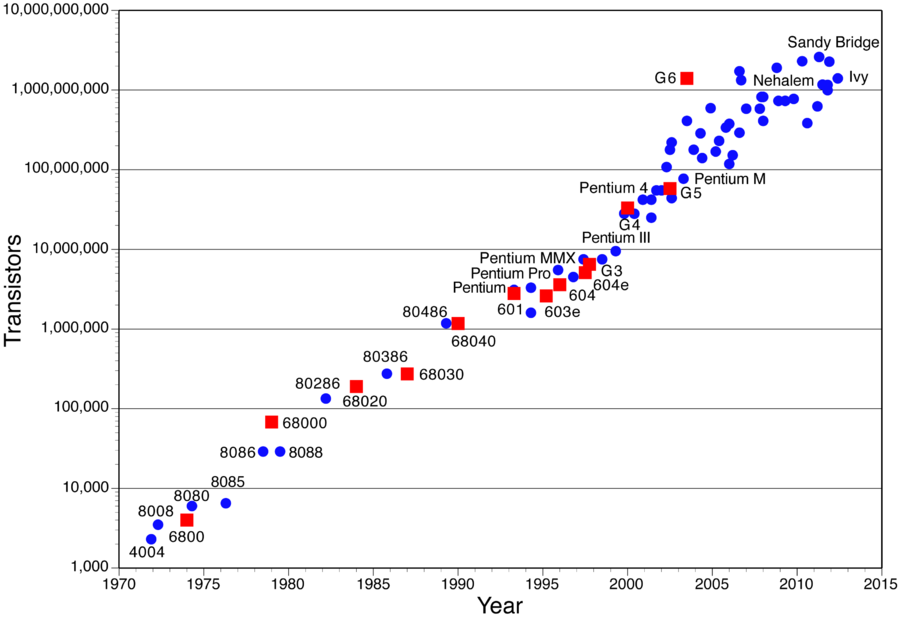
\includegraphics[width=.95\linewidth]{img/02/moorelaw.png} 
        \caption{Nombre de transistor par processeur en fonction du temps.
        Cette croissance exponentielle est connue sous le nom de loi de Moore}
 		\label{fig:moore}
\end{figure}

\begin{figure}[bth]
        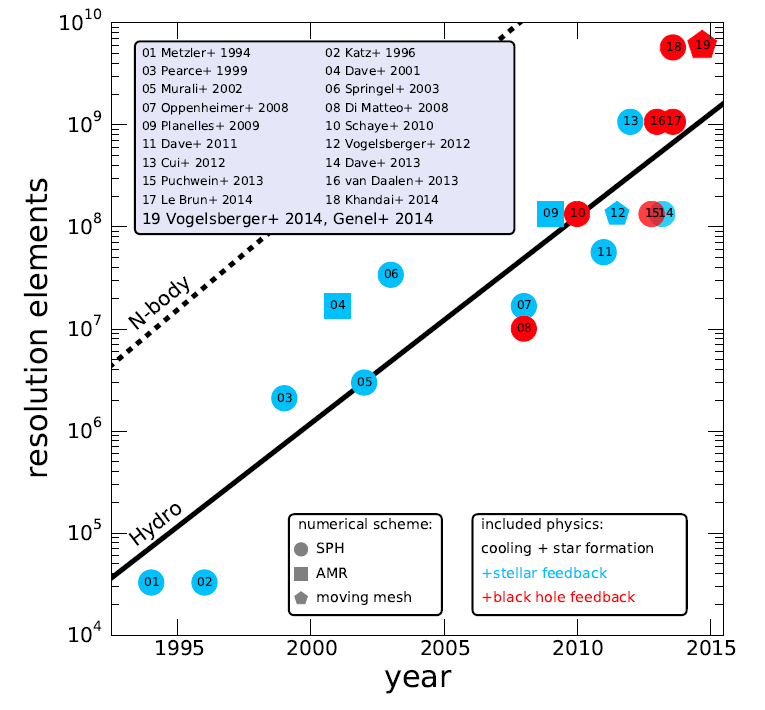
\includegraphics[width=.95\linewidth]{img/02/figure_simulations_with_time.png} 
        \caption{Tailles des simulations en fonction du temps.
        Il existe un lien directe avec la loi de Moore.
         Image illustris}
 		\label{fig:taillesimu}
\end{figure}


\subsection{Principes de parallélisation}

Comme on ne peux pas créer des processeurs aussi gros que ce que l'on le souhaite, la technique utilisée pour continuer a augmenter la puissance de calcul, consiste a en utiliser plusieurs en même temps.
C'est ce qu'on appelle le parallélisme.

Dans le cas des simulation cosmologique, la parallélisation est effectué en découpant l'espace a simuler en un certain nombre de sous domaines.
Chaque processus indépendant sera alors chargé de simuler un sous domaine.
Comme chaque sous domaine n'est pas isolé, mais appartient au même ensemble, les domaines vont devoir communiquer entre eux sur l'état de leurs voisin.
Nous verrons en détail comment est effectué ce découpage dans la section \ref{sec:parasoft}.
Mais voyons d'abord qu'elles sont les contraintes techniques de la parallélisation.

Il existe différent type de parallélisation définis par la taxonomie de Flynn \citep{Flynn:1972:COE:1952456.1952459}: 

\begin{itemize}
\item SISD Single Instructions on Single Data.
Aucun parallélisme, exécution d'une unique série d'instructions sur un unique flux de données.

\item SIMD Single Instructions on Multiple Data.
Exécution d'une unique série d'instructions sur différents flux de données.
C'est le principe de fonctionnement des GPU.

\item MISD Multiple Instructions on Single Data 
Exécution de différentes série d'instructions sur un seul flux de données.

\item MIMD Multiple Instructions on Multiple Data.
Exécution de différentes série d'instructions sur différents flux de données.
C'est l’architecture la plus utilisé aujourd'hui, et celle qui nous intéresse ici.
Le type MIMD est lui même découpé en deux sous ensembles : 

\begin{itemize}
\item On dit que la mémoire est \textit{distribuée} quand les threads on leur propre espace mémoire dédié.
Les principales machines que j'ai pu rencontrer utilise un modèle MIMD a mémoire distribuée.

\item On dit que la mémoire est \textit{partagée} quand plusieurs threads ont accès au mème espace mémoire.
\end{itemize}
\end{itemize}

Il existe plusieurs niveau de parallélisation, au niveau matériel.
Par exemple, un processeur actuel dispose de plusieurs cœurs, capable de géré chacun un processus (voir 2 dans le cas de l'hyperthreading).
Il est possible d'avoir plusieurs processeur au sein d'un même ordinateur.
Et il est possible d'utiliser conjointement plusieurs ordinateurs.
Ce qui nous mène a la notion de centre de calcul.

\subsection{Les calculateurs}

La production de simulation cosmologique a haute valeur scientifique ne se fait pas sur un simple ordinateur personnel.
Pour réaliser de telle simulations, nous (les simulateurs) utilisons des centres de calcul.
A la manière d'un télescope pour les observateurs, les supercalculateur sont les outils principaux des simulateurs.
Et a la manière des plus gros télescopes, ces calculateurs sont gigantesques.

La figure \ref{fig:titan} présente le calculateur TITAN du Oak Ridge Leadership Computing Facility sur lequel ont été éxécuté les simulations CODA \citep{ocvirk_cosmic_2015}.
TITAN a été classé quatrième plus puissant calculateur au monde selon le cite top500.org (cf \ref{tab:top500}).

\begin{figure}[bth]
        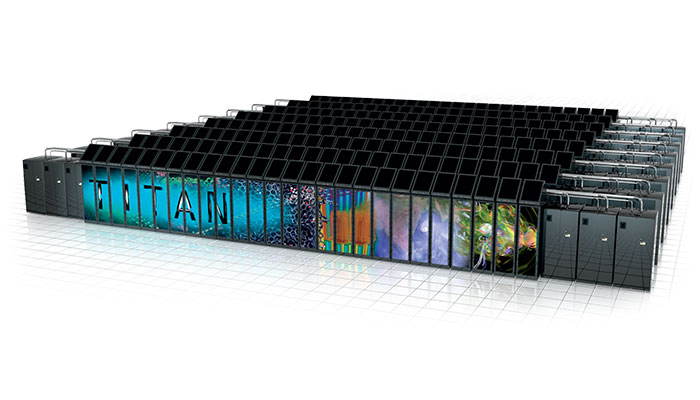
\includegraphics[width=.95\linewidth]{img/02/titan.jpg} 
        \caption{Supercalculateur Titan OLCF.
        ou ont été exécutés les simulations CODA}
 		\label{fig:titan}
\end{figure}

\begin{table}[bth]
\begin{tabular}{ l l l l }
\hline 
Système & Pays & nb de cœurs & TFlop/s (peak) \\
\hline 
Sunway TaihuLight & Chine & 10,649,600 & 125,435.9 \\ 
Tianhe-2  & Chine & 3,120,000 & 54,902.4 \\ 
Piz Daint  & Suisse & 361,760 & 25,326.3 \\ 
Titan  & États unis & 560,640 & 27,112.5 \\ 
Sequoia  & États Unis &1,572,864 & 20,132.7 \\ 
\end{tabular} 
\caption{Les 5 super calculateurs les plus puissants du top500 de Juin 2017, source : www.top500.org}
\label{tab:top500}
\end{table}


Ce type de calculateur est composé d'un certain nombre de nœud (ordinateur) qui communique entre eux par l'intermédiaire d'un réseau.

D'une manière générale, plus des composants sont physiquement éloignés, plus leurs communications seront lente (cf \ref{tab:debits})


\begin{table}
\begin{tabular}{ l l }
\hline 
Interface  & Débit théorique \\
\hline 
Cache L1 & $\approx$ 700Go/s \\
RAM & $\approx$ 20 Go/s \\ 
PCIE 16x & $\approx$ 16 Go/s \\
InfiniBand & $\approx$ 5 Go/s \\
SSD & $\approx$ 600 Mo/s \\
HDD & $\approx$ 100 Mo/s
\end{tabular} 
\caption{Ordre de grandeur des débits théorique des différentes interface rencontrées lors de l'exécution d'un code HPC}
\label{tab:debits}
\end{table}


En principe, la mémoire est partagé au sein d'un nœud, et distribuée sur le réseau.
C'est a dire que tout les processus au sein d'un même nœud pourront communiquer par l'intermédiaire de la RAM, ce type de communications est rapide.
Pour les communications entre les nœuds, l'information devra passer par le réseau, ce type de communications est donc plus lent.
Durant le développement d'un code HPC, on cherchera a minimiser les communications par le réseau.



%Les cœurs au sein d'un même CPU pourront communiquer entre eux de faible quantité de données par l’intermédiaire du cache, ou en passant par la RAM pour les volumes plus importants.



%Proche d'un ordinateur personnel un nœud est composé d'une carte mère sur laquelle est relié entre autres, un ou plusieurs processeurs (CPU), une certaine quantité de mémoire RAM et parfois une carte graphique (GPU)
%Chaque CPU dispose d'un certain nombre de cœurs, et chaque cœurs est capable d'exécuter un certain nombre de processus ou thread (généralement 1, parfois 2 dans le cas de l'Hyperthreading)

%
%Une fois les processus et les domaines identifiés il existe différentes facons de faire dialoguer les processus entre eux.
%La principale distinction viendra généralement de si les threads sont exécutés par un meme noeud ou non.
%
%, cad par exemple que si le thread 0 déclare une variable X, le thread 1 aura aussi accès a cette variable . 
%OpenMP est une API permettant ce  genre partage de mémoire.
%
%
%Si les threads sont exécutés sur un même nœud on aura tendance a utiliser un schéma a base de mémoire partagée.
%
%Dans le cas ou les threads sont exécutés par des processeurs étant physiquement éloigné, ie sur des noeuds différents, les communications doivent passer par un réseau de communication reliant les noeuds.
%Il faudra utiliser dans ce cas une autre API pour explicitement envoyer et recevoir des paquets d'information
%L'API la plus communément utilisée pour ce genre de communication est Message Passing Interface MPI.
%
%
%
%\paragraph{Nœud :} Élément du centre de calcul relier par un réseau.
%
%La difficulté est de géré la façon dont les threads travaillent ensemble.
%En effet a chaque thread sera associé un domaine de calcul représentant une partie de l'espace a modéliser.
%De plus les domaine ne sont pas isolés et partage de l'information. 
%
%Nous sommes alors confronté a plusieurs problèmes: comment associer les threads aux domaines de calculs  et comment faire communiquer ces threads entre eux.
%
%
%
%Ces machines se composent d'un certain nombre de nœuds.



\subsection{Courbe de Peano-Hilbert}
\label{sec:parasoft}

%https://books.google.fr/books?id=sbQqBgAAQBAJ&pg=PA26&lpg=PA26&dq=peano+hilbert+mpi&source=bl&ots=HgSw0Jpf7d&sig=vXTb2JkDixd1gcDGANoARIYHAG0&hl=fr&sa=X&ved=0ahUKEwilofzKoerSAhUF6RQKHXzQDC4Q6AEIGjAA#v=onepage&q=peano%20hilbert%20mpi&f=false


%Warren et Salmon
Le découpage des domaines de calcul correspondants aux différents processeurs, utilise une courbe de Peano-Hilbert.
Ce type de courbes fractale a la particularité de remplir l'espace.
Mais aussi de passer par tout les points d'une grille.
Ainsi si l'on applique ce pavage aux cellules de notre grille, en associant un indice reliant un cellule a sa position sur la courbe de Hilbert.
Il suffit ensuite de découper la courbe en parties identique  pour 
Ainsi si l'on a par exemple  32 cellules a assigner sur 4 processeurs, la courbes sera découpée en 4 parties de 8 cellules.
Chacune de ces partie sera en suite assignée a un processeur.

Ce type de découpage minimise les interfaces entre domaine, en s'assurant d'une proximité spatiale entre tout les points de la courbe.
Elle minimise donc les communications entre processeurs.

\begin{figure}[bth]
        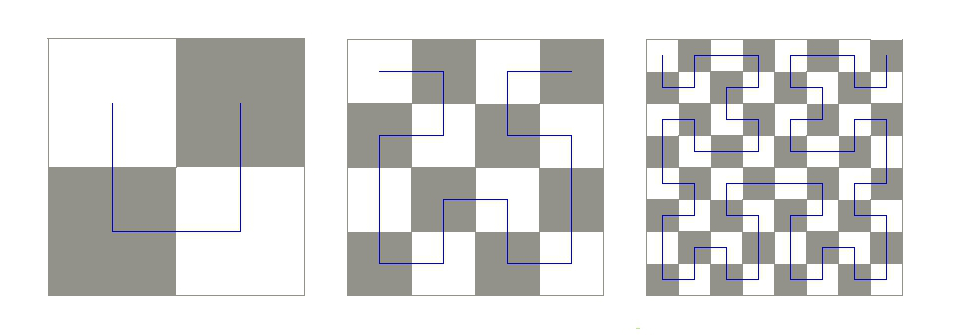
\includegraphics[width=.95\linewidth]{img/02/courbe_Hilbert.jpeg} 
        \caption{exemple de courbe de Hilbert. 
        %http://www.lifl.fr/~pmathieu/transform/fractales.html
}
 		\label{fig:hilbert}
\end{figure}

%
%\begin{figure}[bth]
%        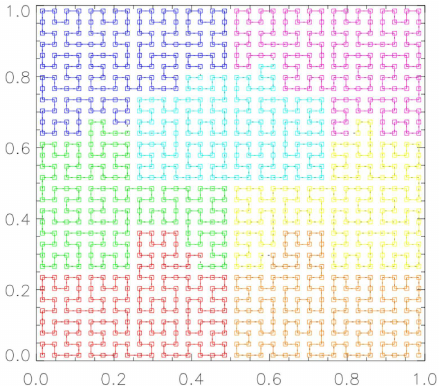
\includegraphics[width=.95\linewidth]{img/02/hilbert2.png} 
%        \caption{exemple de courbe de Hilbert. 
%%http://iopscience.iop.org/article/10.1086/590370/pdf 
%}
% 		\label{fig:hilbert2}
%\end{figure}


Dans l'état actuel du code, la courbe est calculée au debut de la simulation, et donc  seul la grille coarse est prise en compte.
De plus, la repartition des dommaines est statique et n'évolue pas au cour de la simulation.
Dans le cas ou un domaine raffine plus qu'un autre, la charge de travail y est plus importante.
Dans le futur, l'objectif serai de calculer la courbe de Hilbert sur la totalité des cellules feuilles.
Pour ainsi pouvoir refaire le découpage et donc équilibrer la charge entre les processeurs.
C'est ce qui s'appel le "load balancing".


\begin{figure}[bth]
        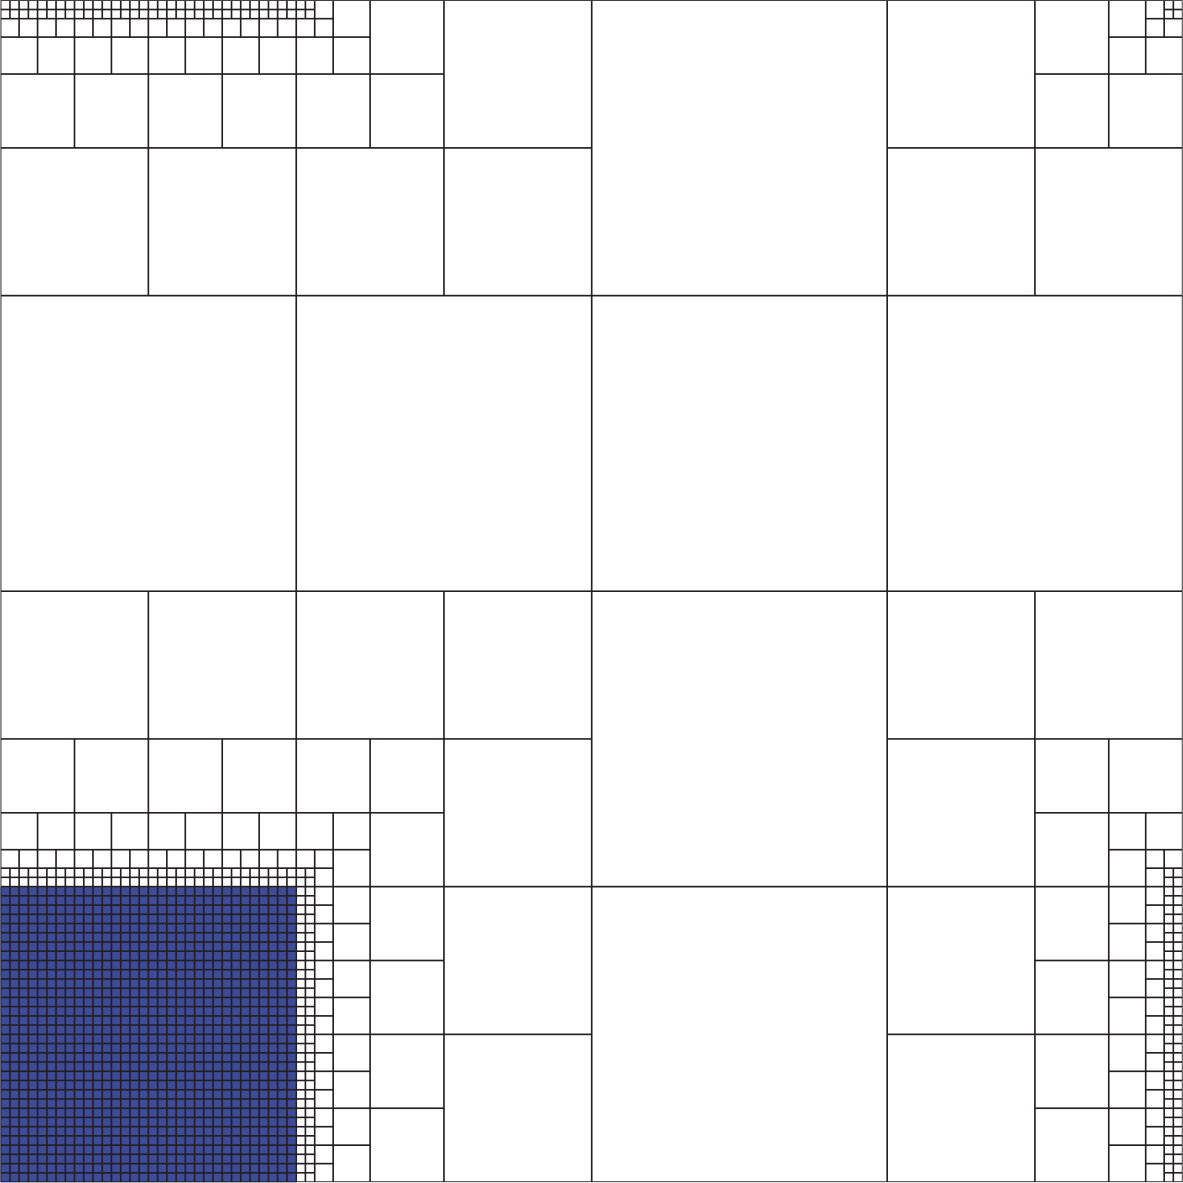
\includegraphics[width=.95\linewidth]{img/02/secteur.png} 
        \caption{Exemple de domaine de processeur généré par EMMA. 
        Chaque domaine représente une vue d'ensemble de la grille, a résolution dégradée.
}
 		\label{fig:hilbert2}
\end{figure}





%Je n'ai aucun doute sur le fait que dans les années a venir 


\subsection{GPU}

EMMA utilise un degré supplémentaire de parallélisation.
Les calcul de chaque domaines sont accéléré en utilisant les capacité parallèle des processeur graphic récents.
Les cartes graphiques, ou GPU (pour Graphics Processing Unit) ont été détourné de leurs utilisation principale d'affichage il y a une dizaine d'années.

A l'inverse des CPU actuels, qui disposent d'un nombre réduit de cœurs (8 coeurs hyperthreadé pour un Intel® Xeon® X7560 de Curie et 16 cœurs pour un AMD Opteron 6300 de TITAN) les GPU dispose d'une nombre beaucoup plus important de coeurs (Fig \ref{fig:cpugpu})
Par exemple la NVIDIA Tesla k40c dispose de 2880 coeurs.

\begin{figure}[bth]
        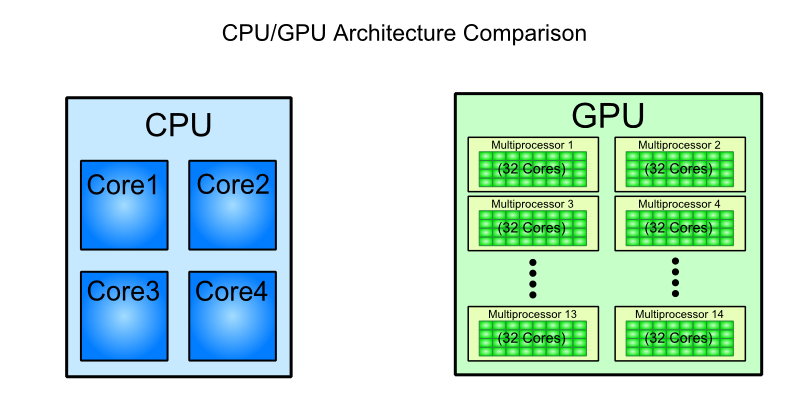
\includegraphics[width=.95\linewidth]{img/02/cpu_vs_gpu.png} 
        \caption{Comparaison CPU/GPU. Une CPU dispose d'un nombre réduit de cœurs capables d’exécuter des opération complexe. A l'inverse un GPU dispose d'un grand nombre de coeurs pouvant éxécuter un grand nombre d'opérations simples en parallèle}
 		\label{fig:cpugpu}
\end{figure}


Un CPU peux exécuter des taches différentes sur chacun de ses coeurs (MIMD).
Les GPU utilise un mode de parallélisation de type SIMD.
Ces unités de calculs sont  efficaces dans le traitement d'un grand nombre d'information en parallèle.
Elle sont donc toutes indiqués dans le cas des simulations numérique ou il s'agit d'appliquer un traitement identique a chaque cellules de la grille.

Il existe 2 principaux avantage aux GPU par rapport aux CPU.
Premièrement leurs meilleurs ratio puissance de calcul sur coup (flop/€).
Et également un meilleur ratio puissance de calcul sur puissance élcetrique (flop/W) ce qui reduit les besoins de refroidissement et permet des économies supplémentaires.


%
% et de 12Go de mémoire et a une puissance de calcul de 4.3 Tflop/s en simple precision.
%
%
%Intel® Xeon® X7560 -> TDP 130 W -> 76 Gflop/s (crete)
%
%
%IBM A2 (sequoia) -> 204 Gflop/s -> TDP 55W

 

Cependant CPU et GPU sont indissociable est il faut les utilisé conjointement pour tirer le meilleurs partis des capacitées de calcul offerte par une machine hybride.

Une code hybride est découpé en deux parties, une partie sequentielle exécuté sur le CPU et une partie paralélle exécuté sur le GPU.
On tirera le maximum des capacités d'accélération d'un GPU avec un code qui est autement parallélisable.
%En effet si l'on peux éspérer



La programmation sur carte graphique utilise une approche proche du concept de mémoire distribuée.
Cad que la carte graphique GPU et le processeur central CPU ont besoin de communiquer.
Leurs espaces mémoire ne sont pas commun.

%Or a l'heure actuelle cette communication utilise une interface relativement lente (PCI express) qui rend coûteuse la communication. 
Il faut donc que la quantité de calcul effectués par la carte soit suffisante pour rentabilisé la communication.


plus dur a programmer, performance dépends du problème.





\subsection{Les communications CPU/GPU}

Les CPU sont capable d'accéder rapidement aux informations en mémoire, quel que soient leurs organisation.
Le GPU sont sensibles à la segmentation des données.
C'est à dire que les calculs sur GPU seront performants si les données sont organisées de facons a ce que leur accés memoire consecutifs soient physiquement proches.
Prenon l'exemple d'une différence finie. 
Pour calculer le nouvel etat d'une cellule, il est necessaire de connaitre sont état actuel, et celui de sa voisine.
L'accès mémoire sera plus rapide si l'information est situer sur un espace mémoire adjacent.

La difficulté est que l'arbre AMR ne respecte pas cette organisation, et peut être extremement fragmenté.
Dans EMMA le choix a été fait d'organiser les données sur le CPU, avant de les envoyer sur le GPU (opération de "gather").
Les calculs sont effectués sur le GPU avec une structure memoire adequate, puis rapatriée et remises dans l'arbre par le CPU ((opération de "scatter") (cf Fig. \ref{fig:gatherscatter})

Ce choix est motivé par le fait qu'une structure mémoire bien organisée peux amener a des gains conséquents.
Par exemple dans ATON %TODO ref
un code de transfert radiatif sur grille fixe, le gain GPU est de l'ordre de 80.

Le pari est ici que la perte de temps genérée par les opérations de gather/scatter sera compensé par l'accélération du GPU.


\begin{figure}[bth]
        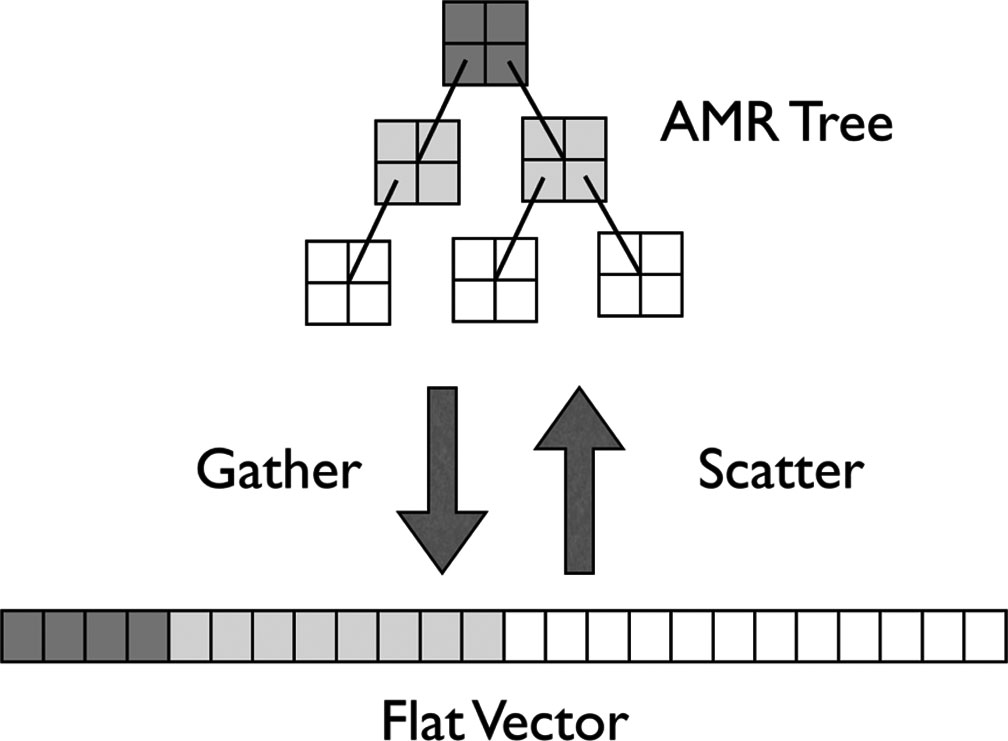
\includegraphics[width=.95\linewidth]{img/02/gatherscatter.jpg} 
        \caption{Transition entre la structure en arbre de l'AMR et la structure en vecteur de calcul.
}
 		\label{fig:gatherscatter}
\end{figure}


En pratique l'opération de gather consiste a rassembler toutes les informations necessaire au calcul de l'état d'une cellule.
Par exemple pour le calcul du potentiel (cf ) %TODO ref
les données necessaires seront: la densité locale, le potentiel local, le potentiel des 6 cellules voisines des axes principaux.
Ces données sont rassemblées dans une structure, et stockées dans un tableau.
Cette opération sera réalisée pour chaque cellule de la grille.

On peut observer ici que les copies ont beaucoup de redondance.
Une cellule d'interet + copie de 6 cellules, le ratio est de $1/6$.
Le potentiel d'une cellule sera copié sept fois sur le GPU.

Ces multiples copies diminue grandements les performances et en font l'une des principales limitations à l'accélération globale du code.
Toute fois, même dans cet état, l'éxécution s'en trouve accélérée d'un facteur $\approx 3$ par rapport à la version CPU.

Dans le but de réduire le nombre de copies et accélérer l'éxécution du code, j'ai modifié les opérations de gather/scatter pour diminuer la redondance des copies.
Au lieu de traiter les cellules unes par unes, l'idée est de traiter les octs.
Dans ce cas les cellules sont traité par 8 et les voisinages au sein d'un oct peuvent être directement traité.
On copie donc 8 cellules d'interet et 4 cellules de bord par face du cube, soit 24 cellules.
Le ratio passe donc a $8/24 = 1/3$ la quantité de copies redondante a donc été diminuée par 2 par rapport au cas précédent.

Vu que la surface d'un cube augmente avec le caré de son coté, alors que son volume augmente avec son cube, plus grand sera la nombre de cellule d'interet, meilleur sera la ratio.
En étendant ce principe, j'ai dévellopé une méthode qui permet de manière récursive d'envoyer une portion d'AMR contenue dans un OCT de niveau arbitraire.

Cependant les résultats ne sont pas a la hauteur des espérances, et l'accélération n'est pas proportionnelle au ratio de données utiles.

IL existe cependant des pistes pour améliorer ce goulot d'étranglement.
La plus prométeuse semble être de suprimer complétement les copies en placant la totalité de l'arbre directement sur la carte.
Dans ce cas, c'est le GPU qui devra gérer l'evolution de l'arbre. 
%Le CPU étant tres efficace pour ce genre d'opération, il semble

Une autre possibilité est de séparer la gestion de l'arbre de la physique.
En l'état actuel, les données physique sont stockées en mémoire avec la même structure que l'arbre.
L'idée serait de stocker dans l'arbre, des indices de cellules permettant de retrouver l'information physique dans des vecteurs plat (cf Fig. \ref{fig:gatherscatter}).
Ainsi les vecteurs pouraient être en premanance sur le GPU, et seul l'information sur leurs position dans l'AMR devrait être transmise.
Un grand nombre de copies seraient alors évitées.



%Copies asynchrones




\subsection{Gestion des entrées sortie}

Si l'on se réfère a la table \ref{tab:debits} on observe que les débits d'accès disques sont les plus faible.
Et étant donné la quantité de données en jeu, une bonne gestion des Entrées/Sorties peut donc permettre un gain de temps appréciable.

Les entrées sorties sont des étapes relativement longues et l'écriture sur disque d'une telle quantité de données demande du temps et ralentit l'exécution de la simulation.
De plus, ces données sont généralement calculé sur des machines distante et leurs rapatriement sur des machine locales peut également être coûteux en temps.
Il a fallu plusieurs mois pour rapatrier localement les données générées par la simulation CODA.

De plus améliorer la compacité des données permet également de gagner du temps au moment du transfert vers des machines distante, ou simplement au moment de la lecture

%analyse a distance

%le feedback CODA\\
%grosse quantité de données\\

Il a fallut plusieurs mois pour rapatrier les données de CODA de TITAN aux états unis vers Strasbourg

CODA II EMMA (voir partie \ref{sec:CODAEMMA})
L'objectif durant ma thèse était de réaliser une simulation de la réionisation avec un nombre de particule de matière noire (et donc une grille coarse) de $2048^3$.
Et si il faut calculer ces données, il faut également les stocker, cad les écrire sur disque dur.

\begin{itemize}
\item Pour les particules:
En considérant qu'un flottant est codé sur 8 bits, chaque champs représente 8Go.
Il y a une dizaine de champs en sortie (3 positions, 3 vitesses, etc): environs 80Go

\item Pour la grille :
En considérant qu'approximativement la quantité de cellule est multipliée pas 3 a cause du raffinement  chaque champ physique (densité, température, composante de la vitesse, etc..) représente environ 24Go de donnée.
Il y a au total un cinquantaine de champs physique nécessaire a l'exécution de la simulation mais en pratique environ une vingtaine en sortie.
Chaque écriture représente donc 500Go pour la grille.

\item Pour les étoiles:
c'est très variable car dépend directement du nombre d'étoile a l'instant donné, qui dépend lui même du paramètre de résolution.
\end{itemize}

Soit au total environ 600Go par pas de temps.

Mais on voudrait évidemment avoir accès a l'état de la simulation a différents instant.
Cette simulation a au final générée 170 snapshot.
Au final le volume de donnée de la simulation représente environs une centaine de tera octets.



Dans l'ancien modèle de données d'EMMA,  
L'intégralité de l'octree était écrit.
Les oct étaient écrit les uns a la suite des autres avec toutes l'information qu'ils contenaient.
L'information étaient exacte, mais le volume de données était considérable.
De plus chaque processeur écrivait un fichier indépendant, ce qui pouvait rapidement faire exploser le nombre de fichiers.


Le nouveau modèle que j'ai implémenté se base sur une notion de tableau de champs.
Les processeurs écrivent conjointement dans le même fichier, le nombre total de fichiers ne dépend plus du nombre de processeurs sur lequel a tourné la simulation.
Les écriture sont réalisées en parallèles grâce a l' utilisation de la librairie hdf5
Selon file-système des calculateurs, il est possible d'avoir un nombre limité de fichier par utilisateur.
Seules les feuilles (les cellules non raffinées) sont écrites sur le disque.
Ce qui permet de réduire la redondance des données, mais ne contrepartie il est nécessaire de reprojeter la grille au niveau voulu 
Chaque fichier représente un champ physique.
Lors d'un transfert entre machine, il est possible de ne rapatrier que les champs nécessaire, et ainsi économiser de la bande passante.
Chaque cellule est considérée comme une particule d'une certaine taille.

%TODO faire le lien avec \ref{fig:gatherscatter}

%Architecture des données 
%conception d'une organisation des données
%séparation des champs
%structure imposé par la gestion de l'AMR
%écriture parallèle

%\subsection{Potentiel d'optimisation EMMA}
%
%la forme des gathers/scatter
%optimisation matérielle -> les prochaines générations de GPU
%Opérations coarse sur grille non AMR.
%reformatage de l'arbre et découplage de la physique




%\begin{figure}[bth]
%        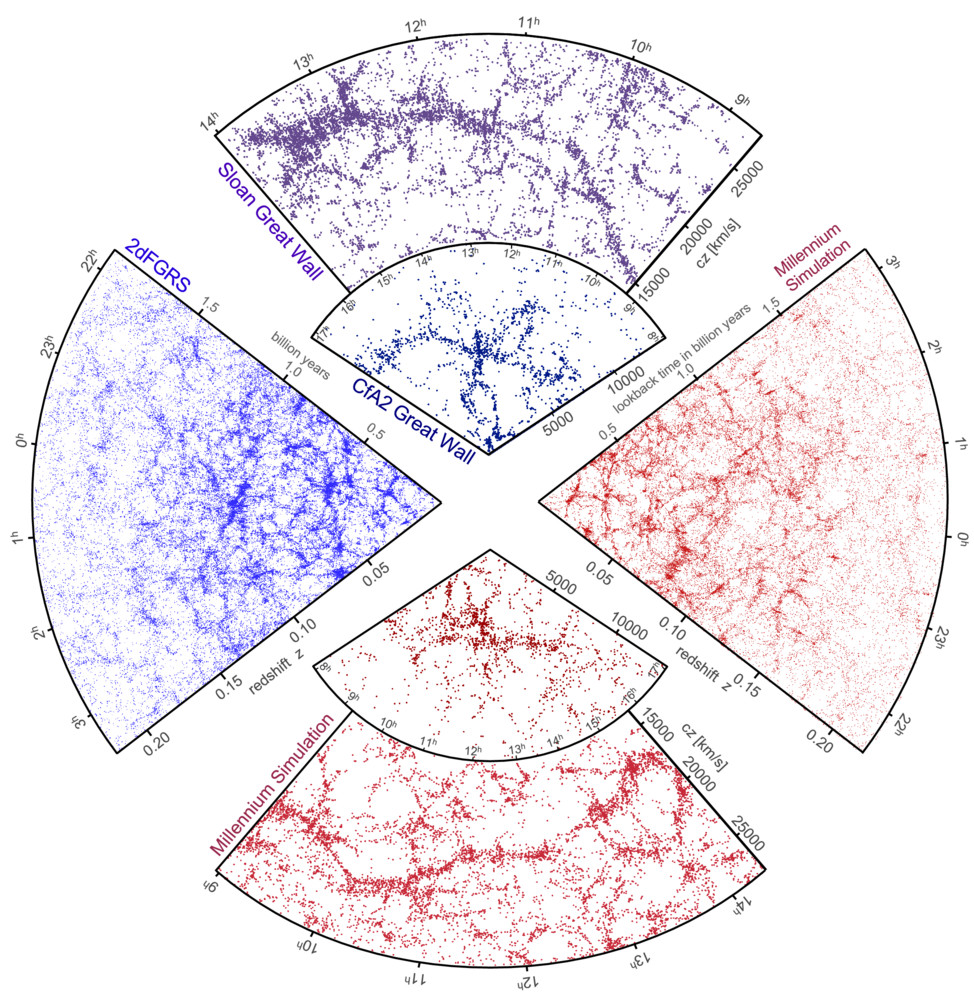
\includegraphics[width=.95\linewidth]{img/02/sdss_millenium.jpeg} 
%        \caption{ 
%%http://wwwmpa.mpa-garching.mpg.de/millennium/
%}
% 		\label{fig:}
%\end{figure}

